% !TEX program = xelatex
% Build:  cd "$DELIV/paper" && tectonic main.tex
% Figures and generated tables:  python3 make_figures.py   (writes fig/*.pdf and gen/*.tex from ../logs)
\documentclass[11pt]{amsart}

%% =====================================================================================
%% HEADLINE NUMBERS.  If a bound improves, edit this block (and rerun make_figures.py so that gen/*.tex and
%% fig/*.pdf are regenerated from the new logs).
%%   Theorem 1.1 (the headline):   m = 14,501. Certified in C: certificate-14501/ (checker rigx.c, BBMST Thm 6.1 tail).
%%                                  Formally verified in Lean: lean/ (checker Checker2Impl at X = 2e9, proof
%%                                  Checker2Math + Checker2Sound + Tail2, root Checker2Sound.not_covers_14501).
%%   Theorem 1.3 (first formalization, Lean):  m = 16,000, logs/, src/rigcert.c and lean/ (root not_covers).
%% Numbers that describe the certified runs are also written out in sections/computation.tex (output lines,
%% cross-checks), sections/evaluation.tex and sections/appendix.tex (command lines, expected output).
%% The numerical observations of Section 7 refer to experiments at m = 16,000 or near m = 14,500 and are
%% written out literally on purpose.
%% =====================================================================================
% --- Theorem 1.1: least modulus <= 14,500 (certificate-14501/output/cert_14501.txt) -------------------
\newcommand{\Mbound}{14{,}500}          % every distinct covering system has least modulus <= \Mbound
\newcommand{\Mzero}{14{,}501}           % distinct moduli all >= \Mzero never cover Z
\newcommand{\MzeroNum}{14501}           % the same number, without the thousands separator
\newcommand{\etaMain}{0.999927}         % certified total for p <= 10^9, rounded up in the 6th decimal
\newcommand{\etaMainTwelve}{0.999926855181}      % certified total as printed (12 digits, an upper bound)
\newcommand{\etaMainFull}{0.99992685518076208}   % the certified double, %.17g
\newcommand{\etaMainHex}{0x1.fff669aac979p-1}    % the certified double, hex
\newcommand{\blockAMain}{0.234899856304}   % primes p < 50
\newcommand{\blockBMain}{0.763569005991}   % primes 50 <= p <= 2e5
\newcommand{\blockCMain}{0.001457990070}   % primes 2e5 < p <= 1e9
\newcommand{\TupMain}{705974.99523353134}  % certified upper bound for T_k
\newcommand{\muLoMain}{7.3144\cdot 10^{-5}}   % <= mu_lo = 7.3144819237924708e-05
\newcommand{\fUpMain}{9.6518\cdot 10^{9}}     % >= f_up = 9651742974.9486885
\newcommand{\critLoMain}{1.5787\cdot 10^{10}} % <= crit_lo = 15787081835.245779
\newcommand{\kPrimesMain}{50{,}847{,}534}  % k = pi(10^9)
\newcommand{\PmaxMain}{10^{9}}             % largest prime treated explicitly
\newcommand{\refEtaLo}{0.99992148081}      % the referee's rigorous interval for the sum of the exact level bounds
\newcommand{\refEtaHi}{0.99992282962}
\newcommand{\runtimeMain}{about $90$ seconds}
% --- Theorem 1.3: least modulus <= 15,999, formally verified (logs/cert16k.txt, lean/) ----------------
\newcommand{\MboundLean}{15{,}999}
\newcommand{\MzeroLean}{16{,}000}
\newcommand{\MzeroLeanNum}{16000}
\newcommand{\etaCert}{0.997385}         % certified total for p <= Pmax, rounded up in the 6th decimal
\newcommand{\etaCertTwelve}{0.997384393974}      % certified total as printed (12 digits, an upper bound)
\newcommand{\etaCertFull}{0.9973843939732947}    % the certified double, %.17g
\newcommand{\etaCertHex}{0x1.fea92ad34fe9cp-1}   % the certified double, hex
\newcommand{\blockA}{0.230571210247}    % primes p < 50
\newcommand{\blockB}{0.760302397508}    % primes 50 <= p <= 2e5
\newcommand{\blockC}{0.006510785610}    % primes 2e5 < p <= 2e8
\newcommand{\Tup}{321051.36453405279}   % certified upper bound for T_k
\newcommand{\TupCeil}{321051.3646}        % a decimal upper bound for \Tup (used in the proof of Theorem 1.3)
\newcommand{\muLo}{0.0026156}           % mu_lo = RD(1 - eta_up) = 0.0026156060267052972 (approx.)
\newcommand{\fUp}{1.2275\cdot 10^{8}}   % >= certified f_up = 122744542.28049764 (upper bound for f_k = T_k/mu_k)
\newcommand{\critLo}{2.8386\cdot 10^{9}} % <= certified crit_lo = 2838631802.0518227 (lower bound for (log k + log log k - 3)^2 k)
\newcommand{\kPrimes}{11{,}078{,}937}   % k = pi(Pmax)
\newcommand{\Pmax}{2\cdot 10^{8}}       % largest prime treated explicitly (m = 16,000)
\newcommand{\PX}{2\cdot 10^{5}}         % largest prime bounded by the comparison bound (m = 16,000); both dumps end here
\newcommand{\tailElem}{0.000849343}     % (100/189) T_up / Pmax, rounded up
\newcommand{\etaElem}{0.998234}         % \etaCertFull + \tailElem, rounded up
\newcommand{\xcheckExact}{0.98120}      % sum over p <= 2e5 of the exact values of the tightest candidate bounds
\newcommand{\xcheckSlack}{0.0097}       % checker's slack over p <= 2e5
\newcommand{\runtimeCert}{about $2.5$ minutes}
\newcommand{\prevBound}{616{,}000}      % BBMST (Invent. Math. 2022)
% Lean checker run (SCRATCH/agents/checkerimpl/full_final.out)
\newcommand{\etaLean}{0.997384786285}
\newcommand{\TupLean}{321095.49941797}
\newcommand{\tailLean}{0.000849458994}
\newcommand{\totalLean}{0.998234245279}
% --- Formal certificate of Theorem 1.1 (lean/MinModulus/Tail2/CertT14501.lean; SCRATCH/agents/lean2/tail2/NOTES.md §4)
% Exact values: numerators over 2^62, printed rounded UP.
\newcommand{\XFormal}{2\cdot10^{9}}           % explicit range of the formal certificate
\newcommand{\etaFormal}{0.999941815948}       % sum of the per-prime costs, p <= 2e9
\newcommand{\etaFormalA}{0.037107790428}      % p < 17 (first moment)
\newcommand{\etaFormalB}{0.961380248462}      % 17 <= p <= 2e5 (S/B/H and tau-split, per prime)
\newcommand{\etaFormalC}{0.001453777059}      % 2e5 < p <= 2e9 (tau-split, blocks)
\newcommand{\TupFormal}{796860.64557339}      % upper bound for T_X, X = 2e9
\newcommand{\tailFormal}{0.000047341491}      % ceil(T * 5941/(50000 X)) / 2^62
\newcommand{\totalFormal}{0.999989157439}     % eta + tail
\newcommand{\slackFormal}{1.08\cdot10^{-5}}
% Intermediate formal certificates (same development): m = 14,600 (X = 2e8, tail of Lemma 4.7) and m = 14,505
% (X = 1e9, tail constant 12473/100000).
\newcommand{\totalLeanTwo}{0.999622630}
\newcommand{\totalLeanThree}{0.99997629}
%% =====================================================================================

\usepackage[margin=1.12in]{geometry}
\usepackage{amsmath,amssymb,amsthm,mathtools}
\usepackage[T1]{fontenc}
\usepackage{lmodern}
\usepackage{microtype}
\usepackage{booktabs}
\usepackage{graphicx}
\usepackage{xcolor}
\usepackage{enumitem}
\usepackage{array}
\usepackage{alltt}
\usepackage{needspace}
\usepackage[colorlinks=true,linkcolor=blue!45!black,citecolor=green!35!black,urlcolor=blue!55!black]{hyperref}
\usepackage[capitalise,nameinlink]{cleveref}

\setlist{itemsep=2pt,topsep=4pt}
\setlength{\emergencystretch}{2em}

% generated macros (derived statistics); see make_figures.py
% generated by make_figures.py -- do not edit
% m = 16,000 certificate
\newcommand{\nPrimesPX}{17{,}984}
\newcommand{\nPrimesCmp}{17{,}974}
\newcommand{\nPrimesMone}{10}
\newcommand{\nPrimesC}{11{,}060{,}953}
\newcommand{\sumCostPX}{0.990874}
\newcommand{\sumMonePX}{16.377278}
\newcommand{\sumBBPX}{2.184877}
\newcommand{\bbPassP}{193}
\newcommand{\bbTotalPX}{2.18}
\newcommand{\gainAmin}{1.25}\newcommand{\gainAmax}{1.31}
\newcommand{\gainBmin}{1.48}\newcommand{\gainBmax}{3.22}
\newcommand{\gainCmin}{3.23}\newcommand{\gainCmax}{10.54}
% m = 14,501 certificate
\newcommand{\nPrimesMoneMain}{6}
\newcommand{\nPrimesSBH}{921}
\newcommand{\nPrimesTauPX}{17{,}057}
\newcommand{\nPrimesCMain}{50{,}829{,}550}
\newcommand{\lastSBH}{7{,}247}
\newcommand{\firstTau}{7{,}253}
\newcommand{\sumCostPXMain}{0.998469}
\newcommand{\sumMonePXMain}{16.743973}
\newcommand{\sumBelowTwoK}{0.914454}
\newcommand{\shareBelowTwoK}{91}
\newcommand{\nKnotsMain}{103}


\theoremstyle{plain}
\newtheorem{theorem}{Theorem}[section]
\newtheorem{lemma}[theorem]{Lemma}
\newtheorem{proposition}[theorem]{Proposition}
\newtheorem{corollary}[theorem]{Corollary}
\newtheorem*{theorem*}{Theorem}
\theoremstyle{definition}
\newtheorem{definition}[theorem]{Definition}
\newtheorem{remark}[theorem]{Remark}
\newtheorem{example}[theorem]{Example}
\newtheorem{observation}[theorem]{Observation}
\crefname{observation}{Observation}{Observations}

\numberwithin{equation}{section}

% notation
\newcommand{\Z}{\mathbb{Z}}
\newcommand{\N}{\mathbb{N}}
\newcommand{\R}{\mathbb{R}}
\newcommand{\E}{\mathbb{E}}
\renewcommand{\P}{\mathbb{P}}
\newcommand{\one}{\mathbf{1}}
\newcommand{\ZZ}[1]{\Z_{#1}}
\newcommand{\pos}[1]{\left(#1\right)^{+}}
\newcommand{\eps}{\varepsilon}
\DeclareMathOperator{\lcm}{lcm}
\DeclareMathOperator{\supp}{supp}
\newcommand{\cF}{\mathcal{F}}
\newcommand{\cA}{\mathcal{A}}
\newcommand{\bk}{\mathbf{k}}
\newcommand{\BBMST}{\cite{BBMST}}
\newcommand{\code}[1]{\texttt{#1}}

\begin{document}

\title[The least modulus of a distinct covering system]{The least modulus of a distinct covering system\\ is at most \Mbound}
\author{Grayson MacKenzie}
\date{\today}

\begin{abstract}
A covering system is a finite collection of congruences $a_i \pmod{d_i}$ whose union is $\Z$. Erd\H{o}s asked
whether the least modulus of a covering system with distinct moduli can be arbitrarily large. Hough showed that
it cannot, with the bound $10^{16}$, and Balister, Bollob\'as, Morris, Sahasrabudhe and Tiba lowered the bound to
$\prevBound$. We prove that congruences with distinct moduli, all at least $\Mzero$, never cover the integers, so
that every covering system with distinct moduli has least modulus at most $\Mbound$.

The proof keeps the distortion method of Balister et al.\ and replaces its second-moment estimate for the loss
at each prime by a comparison theorem: for each of the distorted measures and every convex nondecreasing $\varphi$,
the expectation of $\varphi$ of the number of progressions containing a point is at most its value for aligned
progressions under an explicit tilted product measure. This extends Rogers' theorem on sieving. It bounds the loss at
each prime by an expectation over a random smooth number, which we evaluate exactly, up to explicitly bounded
truncations, by a certified computation in directed rounding. The computation has been cross-checked by independent
code and refereed by an AI agent. The whole proof, including a separate evaluation of the bounds, has also been
formally verified in Lean~4 with Mathlib, modulo one \texttt{native\_decide} evaluation of a numerical checker written in Lean.
\end{abstract}

\maketitle
\setcounter{tocdepth}{1}
\tableofcontents

%% =====================================================================================
\section{Introduction}\label{sec:intro}
%% =====================================================================================

\subsection{Covering systems and the minimum modulus problem}

A \emph{covering system} is a finite collection of arithmetic progressions $a_1+d_1\Z,\dots,a_k+d_k\Z$ whose union
is $\Z$. It is \emph{distinct} if the moduli $d_1,\dots,d_k$ are pairwise distinct. For example,
\[
  0 \bmod 2,\quad 0 \bmod 3,\quad 1 \bmod 4,\quad 5 \bmod 6,\quad 7 \bmod 12
\]
is a distinct covering system with least modulus $2$. Covering systems were introduced by Erd\H{o}s in
1950~\cite{Erdos1950}, who asked whether there are distinct covering systems whose least modulus is arbitrarily
large; this is the \emph{minimum modulus problem}. Explicit constructions push the least modulus up to
$25$ (Gibson~\cite{Gibson2009}), $40$ (Nielsen~\cite{Nielsen2009}) and $42$ (Owens~\cite{Owens2014}), the largest
value known to occur.

In the other direction, Filaseta, Ford, Konyagin, Pomerance and Yu~\cite{FFKPY2007} showed that the sum of the
reciprocals of the moduli of a distinct covering system grows with its least modulus, and in 2015
Hough~\cite{Hough2015} resolved the minimum modulus problem negatively: every distinct covering system has least
modulus at most $10^{16}$. Balister, Bollob\'as, Morris, Sahasrabudhe and Tiba~\cite{BBMST} (henceforth BBMST)
introduced the \emph{distortion method}, which gives a simpler proof of Hough's theorem together with a much
better bound: congruences with distinct moduli, all at least $\prevBound$, do not cover $\Z$
\cite[Theorem~8.1]{BBMST}. The same method proves Schinzel's conjecture and gives lower bounds for the density of
the uncovered set \cite{BBMST}, and it has been used for related questions: the Erd\H{o}s--Selfridge problem for
squarefree moduli \cite{BBMST2021ES}; covering systems with squarefree moduli, where the least modulus is at most
$118$ \cite{CFT2025}; bounds for the $j$-th smallest modulus of a minimal covering system \cite{KKL2024} (see also
\cite{CFT2025}); covering systems whose reciprocal sums are close to $1$ \cite{FilasetaKalogirou2026}; and covering
systems of polynomial rings over finite fields, of global function fields and of number fields
\cite{LWWY2024,LWWY2025,BWang2026,LiWangYi2026}.

\subsection{The main results}

\begin{theorem}\label{thm:main}
Let $d_1,\dots,d_k$ be distinct integers, all at least $\Mzero$, and let $a_1,\dots,a_k\in\Z$. Then there is an
integer $x$ with $x\not\equiv a_i \pmod{d_i}$ for every $i$.
\end{theorem}

\begin{corollary}\label{cor:main}
Every covering system with distinct moduli has least modulus at most $\Mbound$. In particular, the largest least
modulus of a distinct covering system lies between $42$ and $\Mbound$.
\end{corollary}

The previous record was $\prevBound$ \cite{BBMST}. The proof of \cref{thm:main} is computer-assisted, in the limited
and precise sense explained in \cref{sec:intro-computer}. Its numerical part has been certified with outward rounding
and cross-checked by independently written code, and the new parts of the proof and of the computation have been
checked by an independent referee (an AI agent). Moreover, \cref{thm:main}, with the whole of its proof, has been
formally verified in Lean~4 with Mathlib, modulo one \texttt{native\_decide} evaluation of a numerical checker written
in Lean (\cref{sec:lean}). The formal proof evaluates the per-prime bounds in the same way, for the primes up to
$\XFormal$, and replaces the explicit prime-counting estimates behind \cite[Theorem~6.1]{BBMST} by a sharpened
elementary tail estimate (\cref{prop:tailtwo}). An earlier and independent formalization, with a simpler evaluation and
a checker of its own, verified the following weaker statement; its certificate is described in detail in
\cref{sec:certified-lean}.

\begin{theorem}\label{thm:lean}
Congruences with distinct moduli, all at least $\MzeroLean$, do not cover $\Z$. Hence every covering system with
distinct moduli has least modulus at most $\MboundLean$.
\end{theorem}

\subsection{Overview of the method}\label{sec:intro-overview}

Let $\cA$ be a finite family of progressions with distinct moduli, and let $p_1<p_2<\dots<p_n$ be the primes
dividing the lcm of the moduli. The distortion method of BBMST exposes the progressions prime by prime: at level
$i$ it removes the set $B_i$ covered by the progressions whose modulus has largest prime factor $p_i$. Writing
$\Z_{Q_i}=\Z_{Q_{i-1}}\times\Z/p_i^{\gamma_i}$, every point $x$ of $\Z_{Q_{i-1}}$ has a \emph{fibre}, and
$\alpha_i(x)$ denotes the proportion of the fibre covered by $B_i$. Starting from the uniform measure, BBMST build
probability measures $P_1,P_2,\dots$; the measure $P_i$ is obtained from $P_{i-1}$ by moving mass inside each fibre
from the covered to the uncovered points, but never multiplying the mass of a point by more than
$\nu_i=1/(1-\delta_i)$, where $\delta_i\in[0,1)$ is a parameter. The mass that stays on the covered points is the
\emph{loss}
\begin{equation}\label{eq:intro-loss}
  P_i(B_i)=\frac{\E_{P_{i-1}}\bigl[(\alpha_i-\delta_i)^+\bigr]}{1-\delta_i},
\end{equation}
and the progressions do not cover $\Z$ as soon as $\sum_i P_i(B_i)<1$.

BBMST bound the loss by the first and second moments of $\alpha_i$, using $(\alpha-\delta)^+\le\alpha^2/(4\delta)$,
the union bound $\alpha_i\le U$, where $U$ is a weighted count of the progressions through a point, and a bound
on the $P_{i-1}$-measure of a single progression. The quadratic majorant is exact only at $\alpha=2\delta$, and it
charges heavily covered fibres in proportion to $\alpha^2$.

Our main tool is a \emph{comparison theorem} (\cref{thm:comparison}). The distorted measure $P_{i-1}$ is a product
of conditional kernels, each bounded by $\nu_j$ times the uniform density. We show that for every measure of this
kind, every nonnegative combination $U$ of progressions and every convex nondecreasing $\varphi$,
\[
  \E_{P_{i-1}}[\varphi(U)]\le\E\bigl[\varphi(U^{\mathrm{al}})\bigr],
\]
where $U^{\mathrm{al}}$ is obtained by moving all progressions so that they pass through one point, and by
evaluating the resulting count at a random point whose $p_j$-adic valuations $V_j$ are independent with the
\emph{tilted} law $\P(V_j\ge a)=\min(1,\nu_j p_j^{-a})$. Alignment maximizes the overlap of the progressions; for
the uniform measure and $\varphi(u)=(u-1)^+$ the statement is Rogers' theorem on sieving
(\cref{sec:rogers}).

We apply the comparison theorem to the hinge $\varphi(u)=(u-t)^+$ with $0\le t\le\delta_i$. Together with a pointwise
inequality (\cref{lem:pointwise}) and an enlargement of the family to all admissible moduli, which is where the
distinctness of the moduli enters (\cref{lem:enlargement}), it gives the bound (\cref{thm:perprime})
\begin{equation}\label{eq:intro-perprime}
  P_i(B_i)\le\frac{\E\bigl[(U_p(s)-t)^+\bigr]}{1-t},\qquad U_p(s)=\sum_{d\mid s}w_p(d),\qquad
  w_p(d)=\sum_{j\ge1:\,dp^j\ge m}p^{-j},
\end{equation}
where $p=p_i$, $m$ is the least modulus, and $s=\prod_{q<p}q^{v_q}$ is a random $(p-1)$-smooth number with
independent exponents, $\P(v_q\ge a)=\min(1,\nu_q q^{-a})$. The right-hand side depends only on $m$, $p$ and the
parameters $\delta_q$, not on the progressions.

It remains to show that, for $m=\Mzero$ and a suitable choice of the $\delta_q$, the sum over all primes of the
right-hand side of \eqref{eq:intro-perprime} is less than $1$. For every prime $p\le\PmaxMain$ we evaluate it
exactly, up to truncations whose effect is bounded explicitly (\cref{sec:evaluation}): for $p<m/2$ by an identity
that splits the primes below $p$ into three ranges and reduces the expectation to an enumeration and a
two-dimensional law, and for $p>m/2$ by a factorization of the divisor count of $s$. A certified program with
directed rounding shows that the total for $p\le\PmaxMain$ is at most $\etaMain$, and a criterion of BBMST handles
the larger primes (\cref{sec:computation}). The formal proof uses the same evaluation for $p\le\XFormal$ together
with an elementary tail estimate; for $m=\MzeroLean$ a cruder evaluation suffices, and that version was formalized
first. \Cref{fig:cumulative} shows the running
totals. With the distortion parameters of the certificate for $m=\MzeroLean$, the moment bounds of BBMST would
exhaust the whole budget at $p=\bbPassP$.

\subsection{What is new}\label{sec:intro-new}

The comparison theorem extends a classical inequality, and we are careful about what is prior art.
\begin{itemize}
\item \emph{Rogers' theorem} \cite[pp.~242--244]{HalberstamRoth1966} states that, for fixed moduli, the density of
  the integers avoiding the progressions is largest when all the residues are equal. It was proved independently by
  Simpson \cite[Lemma~2.3]{Simpson1986} and was revisited by Tao \cite{TaoRogers2026}, whose compression argument
  has the same structure as our one-coordinate lemma plus induction. Lewis \cite{Lewis1996} and Filaseta et al.
  \cite{FFKPY2007} cite it. It is the case $\nu\equiv1$, unit weights and $\varphi(u)=(u-1)^+$ of
  \cref{thm:comparison}.
\item \emph{Filaseta and Kalogirou} \cite{FilasetaKalogirou2026} used Rogers' theorem (via Lewis) in the
  undistorted stages ($\delta=0$) of a distortion argument, together with the fourth-moment bound
  $(\alpha-\delta)^+\le 27\alpha^4/(256\,\delta^3)$ for the loss. This is prior art for the fractional-moment bounds
  of \cref{sec:theta}.
\item \emph{BBMST's moment lemma} \cite[Lemma~3.6]{BBMST} is the monomial case $\varphi(u)=u^k$ of
  \cref{thm:comparison}, and \cite[Lemma~3.4]{BBMST} is its single-progression case (\cref{sec:bbmst-lemmas}).
\end{itemize}
What is new is the extension in two directions at once: to measures given by $\nu$-bounded product kernels, which
is what makes the inequality applicable to the distorted measures and produces the tilted law; and to the whole
increasing convex order, which allows the non-polynomial hinge $(u-t)^+$. We found no earlier use of convex-order
or tilted comparison inequalities to bound the distortion losses themselves. Two further, minor novelties are the
exact evaluation of the per-prime bounds (\cref{lem:SBH,lem:tausplit}), which is elementary, and an elementary tail
estimate (\cref{prop:tail,prop:tailtwo}) based on Chebyshev's bound for the central binomial coefficient, which can replace
\cite[Theorem~6.1]{BBMST} and Dusart's estimate for the $k$-th prime when the margin is not too small.

\subsection{What is computer-assisted, and what has been checked}\label{sec:intro-computer}

\Cref{thm:criterion} and \cref{prop:bbmst61} reduce \cref{thm:main,thm:lean} to finitely many inequalities between
explicit numbers: the sum over the primes $p\le P_{\max}$ of upper bounds $c_p$ for the expectations in
\eqref{eq:intro-perprime}, together with a term for the larger primes, must be less than $1$. The computer evaluates
these finitely many quantities (for $\kPrimesMain$ primes in the case of \cref{thm:main}) in IEEE double precision
with directed rounding, so that the printed totals are rigorous upper bounds (\cref{sec:rounding}). No search over
covering systems is involved. The distortion parameters were found by floating-point searches, but they are simply
inputs: any choice in $[0,\tfrac12]$ gives a valid bound.

The certificate for \cref{thm:main} has been cross-checked by independently written code, with no violation at any
prime (\cref{sec:xcheck}). An independent referee (an AI agent) checked the new evaluation by hand and by brute force,
audited the rounding and the truncations, and recomputed every per-prime bound up to $\PmaxMain$ with separately
written programs; it found the sum of the exact bounds to lie in $[\refEtaLo,\refEtaHi]$ and found no errors. The
proofs of \cref{thm:main,thm:lean}, each including a separate numerical checker written in Lean, have been formally
verified (\cref{sec:lean}): the only step that is not checked by Lean's kernel is the compiled evaluation of the
checker, which takes about ten minutes for \cref{thm:main}. The certificate for \cref{thm:lean} has also been
reproduced by independent code. \Cref{tab:status} summarizes the status of all results of this paper.

\begin{table}[ht]
\centering
\caption{The results of this paper and how they have been checked. ``Certified'': a computation with outward
rounding; ``cross-checked'': recomputed by independently written code; ``refereed'': checked by an independent AI
agent. No result has yet been refereed by human experts.}
\label{tab:status}
\small
\begin{tabular}{@{}l>{\raggedright\arraybackslash}p{0.38\textwidth}>{\raggedright\arraybackslash}p{0.46\textwidth}@{}}
\toprule
theorem & statement & status\\
\midrule
\ref{thm:main} & least modulus $\le\Mbound$ & certified, cross-checked, refereed; formally verified in Lean~4 (one
  \texttt{native\_decide})\\
\ref{thm:lean} & least modulus $\le\MboundLean$ & certified, cross-checked; formally verified in Lean~4 (one
  \texttt{native\_decide}; an earlier, independent formalization with its own checker)\\
\ref{thm:squarefree} & squarefree moduli: least modulus $\le7$ & certified, recomputed, formally verified in Lean~4
  (one \texttt{native\_decide})\\
\ref{thm:sf23} & squarefree, $23$-smooth moduli $\ge3$ never cover & certified, recomputed exactly by independent
  code, refereed; formally verified in Lean~4 (one \texttt{native\_decide})\\
\ref{thm:sf29} & squarefree, $29$-smooth moduli $\ge3$ never cover & certified, recomputed exactly by independent
  code, refereed; not formalized\\
\ref{thm:sf7type} & squarefree moduli: least modulus $\le6$ (moduli $\ge7$ never cover) & certified,
  recomputed exactly by independent code, refereed; formally verified in Lean~4 ($124$ \texttt{native\_decide}
  evaluations)\\
\ref{thm:sf6smooth} & squarefree, $211$-smooth moduli $\ge6$ never cover & certified, recomputed exactly by
  independent code, refereed; not formalized\\
\ref{thm:odd} & odd moduli: divisibility conditions (A)--(C) & certified, refereed; formally verified in Lean~4 (one
  \texttt{native\_decide} each)\\
\ref{thm:odd2} & six further divisibility conditions & certified, refereed; formally verified in Lean~4 (one
  \texttt{native\_decide} each)\\
\ref{thm:rings} & $\mathbb{F}_q[x]$, genus-$0$ function fields, $\Z[i]$, $\Z[\omega]$ & certified, refereed with
  independent checkers; not formalized\\
\bottomrule
\end{tabular}
\end{table}

\subsection{Organization}

\Cref{sec:distortion} recalls the distortion method. \Cref{sec:comparison} states and proves the comparison theorem
and relates it to Rogers' theorem and to the lemmas of BBMST. \Cref{sec:loss} derives the bound on the loss at one
prime and reduces the theorems to a finite computation. \Cref{sec:evaluation} explains how the bound is evaluated,
and \cref{sec:computation} describes the certified computations, their independent verification and the
formalization. \Cref{sec:limits} discusses which steps of the method are sharp and where the remaining slack lies.
\Cref{sec:further} describes applications to squarefree and odd moduli and to other rings. The appendices list the
distortion schedules, the budgets by prime ranges, the rounding conventions of the checkers and instructions for
reproducing the computations.

\begin{figure}[t]
  \centering
  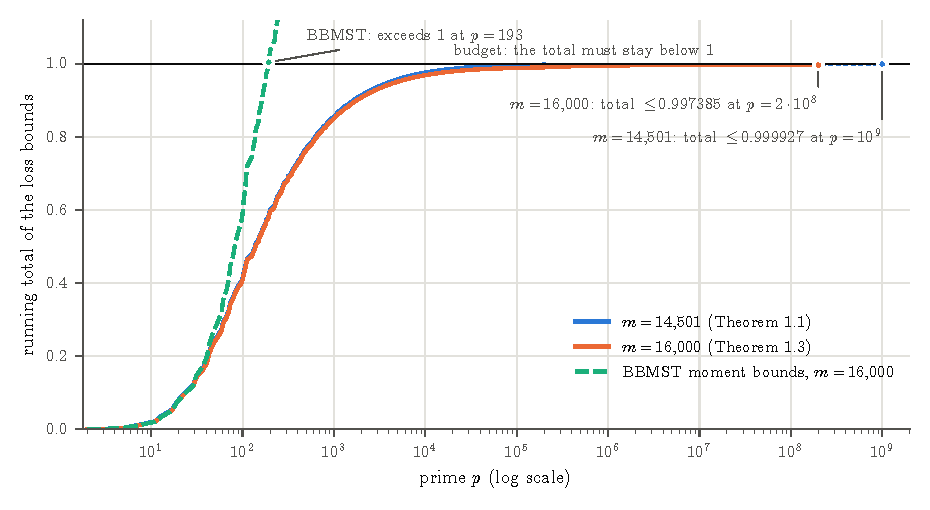
\includegraphics[width=\textwidth]{fig/cumulative_loss.pdf}
  \caption{Running totals of the certified per-prime loss bounds $c_p$ for the certificates of \cref{thm:main}
  ($m=\Mzero$, blue) and of \cref{thm:lean} ($m=\MzeroLean$, orange), for all primes up to $\PX$; beyond, the orange
  curve shows every $20{,}000$-th prime, and the dotted blue segment joins the value at $\PX$ to the certified total
  at $p=\PmaxMain$. The criterion needs the total to stay below $1$. The dashed curve shows the moment bounds
  $b_p=\min\bigl(\E[U_p],\,\E[U_p^2]/(4\delta_p(1-\delta_p))\bigr)$ of BBMST at $m=\MzeroLean$, computed from the
  same certified first and second moments and with the same distortion parameters; their total exceeds $1$ at
  $p=\bbPassP$ and reaches about $2.2$ at $p=\PX$.}
  \label{fig:cumulative}
\end{figure}
% CHECK: logs/xcheck_final.md says the BBMST-type total "reaches 2.19 by 2e5"; recomputing it from
%        logs/dump16k.txt (make_figures.py) gives 2.1849.  The text says "about 2.2", which covers both.

%% =====================================================================================
\section{The distortion method}\label{sec:distortion}
%% =====================================================================================

This section restates the part of the framework of BBMST \cite{BBMST} that we use, in their notation. We give
short proofs, since we use the facts for parameters $\delta_i\in[0,1)$ rather than $[0,\frac12]$, and since the
kernel structure of \cref{lem:kernel} is only implicit in \cite{BBMST}. Results of \cite{BBMST} are cited with
the numbering of the arXiv version (arXiv:1811.03547).
% CHECK: confirm that the numbering of Lemmas 2.1, 2.2, 3.3, 3.4, 3.6, Theorems 3.1, 3.2, 6.1, 8.1 and equations
%        (3)-(5), (13), (19)-(22) is the same in the published version (Invent. Math. 228 (2022) 377-414).

\subsection{Setting}\label{sec:setting}

Let $D$ be a finite set of integers $d\ge2$ and let $\cA=\{A_d:d\in D\}$ with $A_d=a_d+d\Z$. Since $\cA$ is
indexed by $D$, the moduli are distinct. We say that $\cA$ \emph{covers} if $\bigcup_{d\in D}A_d=\Z$. Let
\[
  Q=\lcm(D)=\prod_{j=1}^n p_j^{\gamma_j},\qquad p_1<p_2<\dots<p_n,\qquad \gamma_j\ge1,
\]
and $Q_i=\prod_{j\le i}p_j^{\gamma_j}$ for $0\le i\le n$, so $Q_0=1$ and $Q_n=Q$. We write $\Z_N=\Z/N\Z$. A set
$S\subseteq\Z$ is \emph{$Q_i$-measurable} if it is a union of residue classes modulo $Q_i$; we identify such sets
with subsets of $\Z_{Q_i}$. Let $X_j=\Z/p_j^{\gamma_j}\Z$. By the Chinese remainder theorem,
\[
  \Z_{Q_i}\cong X_1\times\dots\times X_i,\qquad x\mapsto(x\bmod p_1^{\gamma_1},\dots,x\bmod p_i^{\gamma_i}),
\]
and we write $x=(x_1,\dots,x_i)$ and $x_{<j}=(x_1,\dots,x_{j-1})$, which is the reduction of $x$ modulo $Q_{j-1}$.
In particular $\Z_{Q_i}=\Z_{Q_{i-1}}\times X_i$; for $x\in\Z_{Q_{i-1}}$ the \emph{fibre} of $x$ is
$F(x)=\{(x,y):y\in X_i\}$.

The moduli are grouped by their largest prime factor:
\begin{equation}\label{eq:levels}
  N_i=\{d\in D: d\mid Q_i,\ d\nmid Q_{i-1}\},\qquad B_i=\bigcup_{d\in N_i}A_d ;
\end{equation}
thus $N_i$ is the set of moduli whose largest prime factor is $p_i$. This is \cite[(3)]{BBMST}. The set $B_i$ is $Q_i$-measurable. Every $d\in D$ lies in exactly one $N_i$, so
$\bigcup_iB_i=\bigcup_{d\in D}A_d$.

\subsection{The distorted measures}\label{sec:measures}

Fix $\delta_1,\dots,\delta_n\in[0,1)$ and put
\[
  \nu_i=\frac1{1-\delta_i}\ \ge1 .
\]
A probability measure on $\Z_{Q_i}$ is regarded as a measure on $\Z_Q$ by spreading the mass of each residue class
modulo $Q_i$ uniformly over the classes modulo $Q$ that it contains \cite[footnote~2]{BBMST}. In particular, if $P$
is a measure on $\Z_{Q_{i-1}}$, then $P(x,y)=P(x)/|X_i|$ for $(x,y)\in\Z_{Q_i}$. Let $P_0$ be the uniform measure.
Given $P_{i-1}$, BBMST define, for $x\in\Z_{Q_{i-1}}$ \cite[(4)]{BBMST},
\begin{equation}\label{eq:alpha}
  \alpha_i(x)=\frac{\bigl|\{y\in X_i:(x,y)\in B_i\}\bigr|}{|X_i|},
\end{equation}
the proportion of the fibre $F(x)$ covered at level $i$, and \cite[(5)]{BBMST}
\begin{equation}\label{eq:rule}
  P_i(x,y)=
  \begin{cases}
    \max\Bigl(0,\dfrac{\alpha_i(x)-\delta_i}{\alpha_i(x)(1-\delta_i)}\Bigr)\,P_{i-1}(x,y), & (x,y)\in B_i,\\[3mm]
    \min\Bigl(\dfrac1{1-\alpha_i(x)},\dfrac1{1-\delta_i}\Bigr)\,P_{i-1}(x,y), & (x,y)\notin B_i.
  \end{cases}
\end{equation}
The first case occurs only if $\alpha_i(x)>0$ and the second only if $\alpha_i(x)<1$, so \eqref{eq:rule} is well
defined. BBMST take $\delta_i\in[0,\frac12]$. That restriction is used only in their lower bound for the density
of the uncovered set \cite[Lemma~3.5]{BBMST}; the four facts below hold for $\delta_i\in[0,1)$ with the same
proofs. In our application every $\delta_i$ is at most $\frac12$ anyway.

\begin{lemma}[{\cite[Lemma~2.1]{BBMST}}]\label{lem:F1}
For every $x\in\Z_{Q_{i-1}}$ we have $\sum_{y\in X_i}P_i(x,y)=P_{i-1}(x)$. Consequently $P_i(S)=P_{i-1}(S)$ for
every $Q_{i-1}$-measurable set $S$, and $P_n(S)=P_i(S)$ for every $Q_i$-measurable set $S$.
\end{lemma}

\begin{proof}
Write $\alpha=\alpha_i(x)$ and $\delta=\delta_i$, and recall $P_{i-1}(x,y)=P_{i-1}(x)/|X_i|$. If $\alpha\le\delta$,
the covered points receive nothing and the others receive the factor $1/(1-\alpha)$, so the fibre has mass
$(1-\alpha)\cdot\frac1{1-\alpha}P_{i-1}(x)=P_{i-1}(x)$. If $\alpha>\delta$, its mass is
$\bigl(\alpha\cdot\frac{\alpha-\delta}{\alpha(1-\delta)}+(1-\alpha)\frac1{1-\delta}\bigr)P_{i-1}(x)=P_{i-1}(x)$.
Summing over $x$ gives the second statement. If $S$ is $Q_i$-measurable, it is $Q_{j-1}$-measurable for every
$j>i$, and applying the second statement for $j=i+1,\dots,n$ gives $P_n(S)=P_i(S)$.
\end{proof}

\begin{lemma}[{\cite[Lemma~2.2]{BBMST}}]\label{lem:F2}
$P_i(x,y)\le\nu_i\,P_{i-1}(x,y)$ for every $(x,y)\in\Z_{Q_i}$.
\end{lemma}

\begin{proof}
Both factors in \eqref{eq:rule} are at most $1/(1-\delta_i)$, because $(\alpha-\delta)/\alpha\le1$.
\end{proof}

\begin{lemma}[the loss; {\cite[proof of Lemma~3.3]{BBMST}}]\label{lem:F3}
\[
  P_i(B_i)=\frac1{1-\delta_i}\sum_{x\in\Z_{Q_{i-1}}}\bigl(\alpha_i(x)-\delta_i\bigr)^+P_{i-1}(x)
  =\frac{\E_{P_{i-1}}\bigl[(\alpha_i-\delta_i)^+\bigr]}{1-\delta_i}.
\]
\end{lemma}

\begin{proof}
The fibre $F(x)$ contains $\alpha_i(x)|X_i|$ points of $B_i$, each of $P_{i-1}$-mass $P_{i-1}(x)/|X_i|$. By
\eqref{eq:rule} they carry together
$\max\bigl(0,\frac{\alpha_i(x)-\delta_i}{\alpha_i(x)(1-\delta_i)}\bigr)\alpha_i(x)P_{i-1}(x)
=\frac{(\alpha_i(x)-\delta_i)^+}{1-\delta_i}P_{i-1}(x)$ (both sides vanish if $\alpha_i(x)=0$). Sum over $x$.
\end{proof}

\begin{proposition}[the criterion; {\cite[proof of Theorem~3.1, (13)]{BBMST}}]\label{prop:F4}
If $\sum_{i=1}^nP_i(B_i)<1$, then $\cA$ does not cover $\Z$.
\end{proposition}

\begin{proof}
By \cref{lem:F1}, $P_n(B_i)=P_i(B_i)$, since $B_i$ is $Q_i$-measurable. Hence
$P_n\bigl(\bigcup_dA_d\bigr)=P_n\bigl(\bigcup_iB_i\bigr)\le\sum_iP_i(B_i)<1$, so some residue class modulo $Q$ is
not covered.
\end{proof}

\begin{remark}[the rule \eqref{eq:rule} is optimal within each fibre]\label{rem:rule-optimal}
Fix $x$ with $P_{i-1}(x)>0$ and let $P'$ be any measure on $F(x)$ with total mass $P_{i-1}(x)$ and
$P'(x,y)\le\nu_iP_{i-1}(x,y)$ for all $y$; these are the two properties used in
\cref{lem:F1,lem:F2}. The uncovered points of $F(x)$ carry at most $\nu_i(1-\alpha_i(x))P_{i-1}(x)$, so
\[
  P'\bigl(F(x)\cap B_i\bigr)\ \ge\ \Bigl(1-\frac{1-\alpha_i(x)}{1-\delta_i}\Bigr)^+P_{i-1}(x)
  =\frac{(\alpha_i(x)-\delta_i)^+}{1-\delta_i}\,P_{i-1}(x),
\]
which is the value attained by \eqref{eq:rule}. Thus, given $P_{i-1}$, the rule \eqref{eq:rule} minimizes the loss
at level $i$ among all rules with these two properties. (It does not follow that it is optimal for the sum of the
losses over all levels; see \cref{sec:limits}.)
\end{remark}

\subsection{The kernel structure}\label{sec:kernel}

\begin{definition}\label{def:bounded}
Let $X=X_1\times\dots\times X_r$ be a product of finite nonempty sets and let $\nu_1,\dots,\nu_r\ge1$. A
probability measure $\mu$ on $X$ is \emph{$(\nu_1,\dots,\nu_r)$-bounded} if there are \emph{kernels}
$K_j\colon (X_1\times\dots\times X_{j-1})\times X_j\to[0,\infty)$ such that for all $j$ and all $x_{<j}$,
\[
  \sum_{y\in X_j}K_j(x_{<j},y)=1,\qquad K_j(x_{<j},y)\le\frac{\nu_j}{|X_j|}\quad(y\in X_j),
\]
and $\mu(x)=\prod_{j=1}^rK_j(x_{<j},x_j)$ for all $x\in X$.
\end{definition}

In words: under $\mu$, the conditional law of the $j$-th coordinate given the previous ones has density at most
$\nu_j$ with respect to the uniform measure on $X_j$.

\begin{lemma}\label{lem:kernel}
For $1\le i\le n$, the measure $P_{i-1}$, viewed as a measure on $\Z_{Q_{i-1}}=X_1\times\dots\times X_{i-1}$, is
$(\nu_1,\dots,\nu_{i-1})$-bounded.
\end{lemma}

\begin{proof}
For $j\le i-1$ and $x\in\Z_{Q_{i-1}}$ we have $P_{i-1}(x_{\le j})=P_j(x_{\le j})$ by \cref{lem:F1}, where
$P(x_{\le j})$ denotes the mass of the residue class of $x$ modulo $Q_j$. Define
\[
  K_j(x_{<j},x_j)=
  \begin{cases}
    P_j(x_{<j},x_j)/P_{j-1}(x_{<j}) & \text{if } P_{j-1}(x_{<j})>0,\\
    1/|X_j| & \text{otherwise.}
  \end{cases}
\]
By \cref{lem:F1}, $\sum_yK_j(x_{<j},y)=1$. By \cref{lem:F2} and the uniformity of $P_{j-1}$ on fibres,
$P_j(x_{<j},y)\le\nu_jP_{j-1}(x_{<j},y)=\nu_jP_{j-1}(x_{<j})/|X_j|$, so $K_j\le\nu_j/|X_j|$. If
$P_{j-1}(x_{<j})>0$ for all $j\le i-1$, the product $\prod_{j<i}K_j(x_{<j},x_j)$ telescopes to
$P_{i-1}(x)$. Otherwise let $j$ be the least index with $P_{j-1}(x_{<j})=0$; then
$\prod_{l<j}K_l(x_{<l},x_l)=P_{j-1}(x_{<j})=0$, and $P_{i-1}(x)\le P_{i-1}(x_{<j})=P_{j-1}(x_{<j})=0$, so both
sides vanish.
\end{proof}

\subsection{The union bound in the fibre}\label{sec:unionbound}

Every $d\in N_i$ factors uniquely as
\begin{equation}\label{eq:mprime}
  d=m'_d\,p_i^{\,j_d},\qquad p_i\nmid m'_d,\qquad 1\le j_d\le\gamma_i ,
\end{equation}
and $m'_d\mid Q_{i-1}$. Put $A'_d=\{x\in\Z_{Q_{i-1}}:x\equiv a_d\pmod{m'_d}\}$. In coordinates,
\begin{equation}\label{eq:Aprime-cylinder}
  A'_d=\prod_{j<i}\bigl\{x_j\in X_j:\ x_j\equiv a_d \pmod{p_j^{\,v_{p_j}(m'_d)}}\bigr\},
\end{equation}
a product of balls in the sense of \cref{sec:comparison}.

\begin{lemma}[{\cite[proof of Lemma~3.6]{BBMST}}]\label{lem:unionbound}
For every $x\in\Z_{Q_{i-1}}$,
\[
  \alpha_i(x)\le\min\bigl(1,U_i(x)\bigr),\qquad U_i(x)=\sum_{d\in N_i}p_i^{-j_d}\,\one_{A'_d}(x).
\]
\end{lemma}

\begin{proof}
An integer $z$ lies in $A_d$ if and only if $z\equiv a_d\pmod{m'_d}$ and $z\equiv a_d\pmod{p_i^{j_d}}$. Hence the
fibre $F(x)$ meets $A_d$ in $p_i^{\gamma_i-j_d}$ points if $x\in A'_d$ and in no point otherwise. Divide by
$|X_i|=p_i^{\gamma_i}$ and use the union bound; trivially $\alpha_i\le1$.
\end{proof}

\subsection{The moment bounds of BBMST}\label{sec:bbmst-moments}

For comparison we record the bounds of \cite{BBMST}. Let $M_i^{(k)}=\E_{P_{i-1}}[\alpha_i^k]$ and
$\nu(d)=\prod_{p_j\mid d}\nu_j$ for $d\mid Q$ \cite[(8)]{BBMST}.

\begin{lemma}[{\cite[Lemma~3.3]{BBMST}}]\label{lem:bbmst33}
If $0<\delta_i<1$, then $P_i(B_i)\le\min\bigl(M_i^{(1)},\,M_i^{(2)}/(4\delta_i(1-\delta_i))\bigr)$.
\end{lemma}

The first bound follows from $P_i\le P_{i-1}$ on $B_i$, the second from \cref{lem:F3} and
$(\alpha-\delta)^+\le\alpha^2/(4\delta)$. BBMST bound the moments via \cref{lem:unionbound} and the estimate
$P_{i-1}(b+d\Z)\le\nu(\gcd(d,Q_{i-1}))/d$ \cite[Lemma~3.4]{BBMST}, which gives \cite[Lemma~3.6]{BBMST}
\begin{equation}\label{eq:bbmst36}
  M_i^{(k)}\le\sum_{d_1,\dots,d_k\in N_i}p_i^{-(j_{d_1}+\dots+j_{d_k})}\,
  \frac{\nu\bigl(\lcm(m'_{d_1},\dots,m'_{d_k})\bigr)}{\lcm(m'_{d_1},\dots,m'_{d_k})},
\end{equation}
and \cite[Theorem~3.2]{BBMST}, valid for $\delta_j\in[0,\frac12]$,
\begin{equation}\label{eq:bbmst32}
  M_i^{(2)}\le\frac1{(p_i-1)^2}\prod_{j<i}\Bigl(1+\frac{\nu_j(3p_j-1)}{(p_j-1)^2}\Bigr).
\end{equation}
\Cref{thm:comparison} below reproves \eqref{eq:bbmst36} (\cref{sec:bbmst-lemmas}), and \cref{sec:loss} replaces
the second-moment bound by the hinge.

%% =====================================================================================
\section{The comparison theorem}\label{sec:comparison}
%% =====================================================================================

\subsection{Statement}\label{sec:comparison-statement}

Throughout this section $X=X_1\times\dots\times X_n$ with $X_i=\Z/q_i^{e_i}\Z$, where $q_i\ge2$ and $e_i\ge0$ are
integers; in our application the $q_i$ are distinct primes. A \emph{ball of depth $a$} in $X_i$
($0\le a\le e_i$) is a set $\{y\in X_i: y\equiv c\pmod{q_i^{a}}\}$; it has $q_i^{e_i-a}$ elements. A
\emph{cylinder} is a product $C=C_1\times\dots\times C_n$ of balls; we write $a_i(C)$ for the depth of $C_i$. When
the $q_i$ are pairwise coprime, the Chinese remainder theorem identifies the cylinders with the residue classes
$c+L\Z$, $L\mid\prod_iq_i^{e_i}$, and then $a_i(C)=v_{q_i}(L)$.

\begin{definition}[the tilted law]\label{def:tilted}
Let $q\ge2$ be an integer and $\nu\ge1$. A random variable $V$ with values in $\{0,1,2,\dots\}$ has the
\emph{$(q,\nu)$-tilted law} if
\[
  \P(V\ge a)=\min\bigl(1,\nu q^{-a}\bigr)\qquad(a=0,1,2,\dots).
\]
If $\nu\le q$, this means $\P(V=0)=1-\nu/q$ and $\P(V=a)=\nu q^{-a}(1-1/q)$ for $a\ge1$. For $\nu=1$ it is the
law of the $q$-adic valuation of a Haar-random $q$-adic integer.
\end{definition}

\begin{theorem}[comparison theorem]\label{thm:comparison}
Let $\mu$ be a $(\nu_1,\dots,\nu_n)$-bounded probability measure on $X$ (\cref{def:bounded}), let $\cF$ be a finite
family of cylinders with weights $w_C\ge0$, and let $U=\sum_{C\in\cF}w_C\one_C$. Let $V_1,\dots,V_n$ be
independent, $V_i$ with the $(q_i,\nu_i)$-tilted law, and define the \emph{aligned count}
\[
  U^{\mathrm{al}}=\sum_{C\in\cF}w_C\prod_{i=1}^n\one\{V_i\ge a_i(C)\}.
\]
Then for every convex nondecreasing function $\varphi\colon[0,\infty)\to\R$,
\[
  \E_\mu\bigl[\varphi(U)\bigr]\le\E\bigl[\varphi(U^{\mathrm{al}})\bigr].
\]
\end{theorem}

Recall that a random variable $A$ is dominated by $B$ in the \emph{increasing convex order} if
$\E\varphi(A)\le\E\varphi(B)$ for all convex nondecreasing $\varphi$ for which the expectations exist.
\Cref{thm:comparison} says that the law of $U$ under $\mu$ is dominated in this order by the law of
$U^{\mathrm{al}}$. The name comes from the following description of $U^{\mathrm{al}}$. Translate every cylinder
$C$ so that it contains $0$; the translate is $C^0=\{x:\ q_i^{a_i(C)}\mid x_i\ \text{for all } i\}$, and
$\one_{C^0}(x)=\prod_i\one\{v_{q_i}(x_i)\ge a_i(C)\}$. Thus $U^{\mathrm{al}}$ is the value of the aligned
configuration $\sum_Cw_C\one_{C^0}$ at a random point whose coordinates have independent valuations with the tilted
laws. For $\nu_i=1$ this random point is uniform, and for $\nu_i>1$ it is tilted towards $0$, where the aligned
cylinders overlap the most.

We first prove the theorem for the hinge functions $\varphi(u)=(u-t)^+$, by induction over the coordinates
(\cref{sec:onecoord,sec:proof}); the general case follows because the hinges generate the increasing convex order
(\cref{lem:hinges}).

\subsection{The one-coordinate lemma}\label{sec:onecoord}

For an integer $N\ge1$ and a real $\nu\ge1$ define the \emph{greedy weights}
\[
  g_{\nu,N}(k)=\min\bigl(\nu,\max(0,N-\nu k)\bigr),\qquad k=0,1,\dots,N-1 .
\]

\begin{lemma}\label{lem:greedy}
The weights $g=g_{\nu,N}$ are nonincreasing, lie in $[0,\nu]$, and satisfy $\sum_{k<M}g(k)=\min(\nu M,N)$ for
$0\le M\le N$. In particular $\sum_{k<N}g(k)=N$. More precisely, with $J=\lfloor N/\nu\rfloor\le N$, we have
$g(k)=\nu$ for $k<J$, $g(J)=N-\nu J\in[0,\nu)$ if $J<N$, and $g(k)=0$ for $J<k<N$.
\end{lemma}

\begin{proof}
For $k<J$ we have $k\le N/\nu-1$, so $N-\nu k\ge\nu$. For $k>J$ we have $k\ge J+1>N/\nu$, so $N-\nu k<0$. This
gives the explicit form, and the partial sums follow: they equal $\nu M$ for $M\le J$ and $\nu J+(N-\nu J)=N$ for
$M>J$, while $\nu M\le N$ exactly when $M\le J$.
\end{proof}

\begin{lemma}[one coordinate]\label{lem:onecoord}
Let $Y$ be a finite set with $N=|Y|$, let $\nu\ge1$, and let $\kappa\colon Y\to[0,\nu]$ satisfy
$\sum_{y\in Y}\kappa(y)=N$. Let $(B_l)_{l\in L}$ be finitely many subsets of $Y$ with weights $w_l\ge0$, and put
\[
  F(y)=\sum_lw_l\one_{B_l}(y)\quad(y\in Y),\qquad G(k)=\sum_lw_l\one\{k<|B_l|\}\quad(0\le k<N).
\]
Then for every $t\in\R$,
\[
  \sum_{y\in Y}\kappa(y)\bigl(F(y)-t\bigr)^+\le\sum_{k=0}^{N-1}g_{\nu,N}(k)\bigl(G(k)-t\bigr)^+ .
\]
\end{lemma}

\begin{proof}
The proof has three steps.

\emph{(a) Majorization.} For every $s\in\R$,
\begin{equation}\label{eq:majorization}
  \sum_{y\in Y}(F(y)-s)^+\le\sum_{k<N}(G(k)-s)^+ .
\end{equation}
Let $S=\{y:F(y)>s\}$ and $M=|S|$. Since $\sum_{k<M}\one\{k<|B_l|\}=\min(M,|B_l|)\ge|S\cap B_l|$,
\begin{align*}
  \sum_y(F(y)-s)^+&=\sum_{y\in S}(F(y)-s)=\sum_lw_l|S\cap B_l|-sM\\
  &\le\sum_lw_l\min(M,|B_l|)-sM=\sum_{k<M}(G(k)-s),
\end{align*}
and the right-hand side is at most $\sum_{k<N}(G(k)-s)^+$.

\emph{(b) Duality.} For every $\lambda\ge0$,
\begin{equation}\label{eq:duality}
  \sum_y\kappa(y)(F(y)-t)^+\le\lambda N+\nu\sum_y(F(y)-t-\lambda)^+ .
\end{equation}
Indeed $a^+\le\lambda+(a-\lambda)^+$ for every real $a$ and $\lambda\ge0$; multiply by $\kappa(y)\in[0,\nu]$, sum
over $y$ and use $\sum_y\kappa(y)=N$.

\emph{(c) Choice of $\lambda$.} Let $h_k=(G(k)-t)^+$. Since $G$ is nonincreasing, so is $h$. For $\lambda\ge0$
we have $(G(k)-t-\lambda)^+=(h_k-\lambda)^+$. Let $J=\lfloor N/\nu\rfloor$ as in \cref{lem:greedy}. If $J=N$, then
$\nu=1$ and $g\equiv1$; take $\lambda=0$ in \eqref{eq:duality} and apply \eqref{eq:majorization} with $s=t$. If
$J<N$, take $\lambda=h_J$. By \eqref{eq:duality} and then \eqref{eq:majorization} with $s=t+\lambda$,
\begin{align*}
  \sum_y\kappa(y)(F(y)-t)^+&\le\lambda N+\nu\sum_{k<N}(h_k-\lambda)^+
  =h_JN+\nu\sum_{k<J}(h_k-h_J)\\
  &=(N-\nu J)h_J+\sum_{k<J}\nu h_k=\sum_{k<N}g(k)h_k,
\end{align*}
because $h_k\ge h_J$ for $k<J$ and $h_k\le h_J$ for $k\ge J$.
\end{proof}

\begin{remark}\label{rem:lp}
The right-hand side of \cref{lem:onecoord} is the maximum of the linear functional
$\kappa'\mapsto\sum_k\kappa'_kh_k$ over $\kappa'\in[0,\nu]^N$ with $\sum_k\kappa'_k=N$: since $h$ is nonincreasing,
the greedy vector $g$ is optimal (the bathtub principle), and $\lambda=h_J$ is an optimal dual variable. The lemma
thus combines two extremal facts: the worst density puts the maximal weight $\nu$ on the most covered points, and
the worst arrangement of the sets $B_l$ nests them into initial segments of a single ordering of $Y$.
\end{remark}

\subsection{Proof of the comparison theorem}\label{sec:proof}

We first prove a version for arbitrary product sets, in which only the sizes of the sets enter.

\begin{proposition}[rectangle form]\label{prop:rectangles}
Let $X=X_1\times\dots\times X_n$ be a product of finite nonempty sets, $N_i=|X_i|$, and let $\mu$ be a
$(\nu_1,\dots,\nu_n)$-bounded probability measure on $X$. Let $(R_c)_{c\in I}$ be finitely many rectangles
$R_c=R_{c,1}\times\dots\times R_{c,n}$ with $R_{c,i}\subseteq X_i$, with weights $w_c\ge0$, and let
$U=\sum_cw_c\one_{R_c}$. Let $\bk_1,\dots,\bk_n$ be independent random variables with
$\P(\bk_i=k)=g_{\nu_i,N_i}(k)/N_i$ for $0\le k<N_i$. Then for every $t\in\R$,
\[
  \E_\mu\bigl[(U-t)^+\bigr]\le\E\Bigl[\Bigl(\sum_cw_c\prod_{i=1}^n\one\{\bk_i<|R_{c,i}|\}-t\Bigr)^+\Bigr].
\]
\end{proposition}

\begin{proof}
Induction on $n$. For $n=0$ the space is a point and both sides equal $(\sum_cw_c-t)^+$. Let $n\ge1$, put
$X'=X_1\times\dots\times X_{n-1}$ and write points of $X$ as $(x',y)$ with $y\in X_n$. By
\cref{def:bounded}, $\mu(x',y)=\mu'(x')K_n(x',y)$, where $\mu'(x')=\prod_{j<n}K_j(x_{<j},x_j)$ is a
$(\nu_1,\dots,\nu_{n-1})$-bounded probability measure on $X'$. Write $R_c=R'_c\times R_{c,n}$.

Fix $x'\in X'$. As a function of $y$,
$U(x',y)=\sum_c\bigl(w_c\one_{R'_c}(x')\bigr)\one_{R_{c,n}}(y)$ is a nonnegative combination of the sets
$R_{c,n}\subseteq X_n$, and $\kappa=N_nK_n(x',\cdot)$ takes values in $[0,\nu_n]$ and sums to $N_n$.
\Cref{lem:onecoord} gives
\[
  \sum_yK_n(x',y)\bigl(U(x',y)-t\bigr)^+\le\sum_k\P(\bk_n=k)\bigl(U^{(k)}(x')-t\bigr)^+,\qquad
  U^{(k)}=\sum_c\bigl(w_c\one\{k<|R_{c,n}|\}\bigr)\one_{R'_c}.
\]
Multiply by $\mu'(x')$, sum over $x'$ and exchange the finite sums:
\[
  \E_\mu\bigl[(U-t)^+\bigr]\le\sum_k\P(\bk_n=k)\,\E_{\mu'}\bigl[(U^{(k)}-t)^+\bigr].
\]
For each $k$, $U^{(k)}$ is a nonnegative combination of rectangles in $X'$, so by the induction hypothesis
$\E_{\mu'}[(U^{(k)}-t)^+]\le\E\bigl[\bigl(\sum_cw_c\one\{k<|R_{c,n}|\}\prod_{i<n}\one\{\bk_i<|R_{c,i}|\}-t\bigr)^+\bigr]$.
Averaging over $k$ with the weights $\P(\bk_n=k)$, and using the independence of $\bk_n$ from
$(\bk_i)_{i<n}$, gives the claim.
\end{proof}

\begin{lemma}[the tilted law]\label{lem:vlaw}
Let $N=q^e$, $\nu\ge1$, and let $\bk$ have law $\P(\bk=k)=g_{\nu,N}(k)/N$. Define
$V=\max\{a\in\{0,\dots,e\}:\bk<q^{e-a}\}$. Then $\{V\ge a\}=\{\bk<q^{e-a}\}$ and
$\P(V\ge a)=\min(1,\nu q^{-a})$ for $0\le a\le e$. Consequently $V$ has the law of $\min(V^\infty,e)$, where
$V^\infty$ has the $(q,\nu)$-tilted law, and $\one\{\bk<|B|\}=\one\{V\ge a\}$ for every ball $B$ of depth $a$.
\end{lemma}

\begin{proof}
The events $E_a=\{\bk<q^{e-a}\}$ decrease in $a$ and $E_0$ is certain, so $V$ is well defined and
$\{V\ge a\}=E_a$. By \cref{lem:greedy}, $\P(E_a)=\min(\nu q^{e-a},N)/N=\min(1,\nu q^{-a})$. The variables $V$ and
$\min(V^\infty,e)$ take values in $\{0,\dots,e\}$ and have the same tails there, hence the same law. A ball of
depth $a$ has $q^{e-a}$ elements.
\end{proof}

\begin{lemma}[hinges suffice]\label{lem:hinges}
Let $A$ and $B$ be random variables that take finitely many values, all in $[0,\infty)$. If
$\E(A-t)^+\le\E(B-t)^+$ for every $t\ge0$, then $\E\varphi(A)\le\E\varphi(B)$ for every convex nondecreasing
$\varphi\colon[0,\infty)\to\R$.
\end{lemma}

\begin{proof}
Let $0=s_0<s_1<\dots<s_r$ be the elements of $\{0\}\cup A(\Omega)\cup B(\Omega)$; if $r=0$ there is nothing to prove.
Let $\sigma_0=0$ and $\sigma_j=(\varphi(s_j)-\varphi(s_{j-1}))/(s_j-s_{j-1})$ for $1\le j\le r$. Since $\varphi$ is
nondecreasing and convex, $0\le\sigma_1\le\dots\le\sigma_r$. The function
\[
  \psi(u)=\varphi(0)+\sum_{j=1}^r(\sigma_j-\sigma_{j-1})(u-s_{j-1})^+
\]
has slope $\sigma_k$ on $[s_{k-1},s_k]$ and $\psi(0)=\varphi(0)$, so $\psi(s_j)=\varphi(s_j)$ for all $j$. Hence
\begin{align*}
  \E\varphi(A)=\E\psi(A)&=\varphi(0)+\sum_j(\sigma_j-\sigma_{j-1})\E(A-s_{j-1})^+\\
  &\le\varphi(0)+\sum_j(\sigma_j-\sigma_{j-1})\E(B-s_{j-1})^+=\E\varphi(B),
\end{align*}
because every coefficient $\sigma_j-\sigma_{j-1}$ is nonnegative.
\end{proof}

\begin{proof}[Proof of \cref{thm:comparison}]
Apply \cref{prop:rectangles} to the cylinders $R_C=C$. For each $i$ let $W_i=\max\{a\le e_i:\bk_i<q_i^{e_i-a}\}$ as in
\cref{lem:vlaw}. Then $\one\{\bk_i<|C_i|\}=\one\{W_i\ge a_i(C)\}$, the $W_i$ are independent, and $W_i$ has the law
of $\min(V_i,e_i)$. Hence the right-hand side of \cref{prop:rectangles} equals
$\E\bigl[\bigl(\sum_Cw_C\prod_i\one\{\min(V_i,e_i)\ge a_i(C)\}-t\bigr)^+\bigr]$. Since $a_i(C)\le e_i$, we have
$\one\{\min(V_i,e_i)\ge a_i(C)\}=\one\{V_i\ge a_i(C)\}$, and therefore $\E_\mu[(U-t)^+]\le\E[(U^{\mathrm{al}}-t)^+]$ for
every $t\in\R$. Both $U$ and $U^{\mathrm{al}}$ take finitely many nonnegative values, and \cref{lem:hinges} completes
the proof.
\end{proof}

\subsection{Sharpness}

\begin{proposition}\label{prop:sharp}
Suppose that every cylinder of $\cF$ contains $0$. Then there is a $(\nu_1,\dots,\nu_n)$-bounded measure $\mu$ for
which equality holds in \cref{thm:comparison} for every $\varphi$.
\end{proposition}

\begin{proof}
The balls of $X_i$ that contain $0$ are the sets $q_i^aX_i$, and they are nested. Hence there is an enumeration
$\pi_i\colon\{0,\dots,N_i-1\}\to X_i$ such that $\pi_i(\{k:k<q_i^{e_i-a}\})=q_i^aX_i$ for every $a$: list $0$ first,
then the elements of valuation $e_i-1$, then those of valuation $e_i-2$, and so on. Let
$K_i(x_{<i},\pi_i(k))=g_{\nu_i,N_i}(k)/N_i$, independently of $x_{<i}$. Under the product measure $\mu$ the vector
$(\pi_i^{-1}(x_i))_i$ has the law of $(\bk_i)_i$, and $\one_C(x)=\prod_i\one\{\pi_i^{-1}(x_i)<|C_i|\}$ for
$C\in\cF$. By \cref{lem:vlaw}, $U$ has the law of $U^{\mathrm{al}}$.
\end{proof}

So the comparison theorem loses nothing by itself: the extremal measure puts the maximal density $\nu_i$ on the
points of highest valuation, and the extremal configuration is the aligned one.

\subsection{Rogers' theorem}\label{sec:rogers}

\begin{corollary}[Rogers \cite{HalberstamRoth1966}; Simpson \cite{Simpson1986}]\label{cor:rogers}
Let $d_1,\dots,d_k$ be positive integers, not necessarily distinct, and let $a_1,\dots,a_k\in\Z$. Then the density
of $\bigcup_i(a_i+d_i\Z)$ is at least the density of $\bigcup_id_i\Z$. Equivalently, for fixed moduli the density
of the integers that avoid all the progressions is largest when all the residues are $0$.
\end{corollary}

\begin{proof}
Let $L=\lcm(d_1,\dots,d_k)=\prod_jq_j^{e_j}$ and $X=\prod_j\Z/q_j^{e_j}$, identified with $\Z_L$; the uniform measure
$\mu$ is $(1,\dots,1)$-bounded, and each progression $a_i+d_i\Z$ is a cylinder $C_i$ of depths $v_{q_j}(d_i)$. Let
$U=\sum_i\one_{C_i}$. Since $U$ is integer-valued, the indicator of the union is $\min(1,U)=U-(U-1)^+$, so the
density of the union is $\E_\mu U-\E_\mu(U-1)^+=\sum_i1/d_i-\E_\mu(U-1)^+$. By \cref{thm:comparison} with
$\varphi(u)=(u-1)^+$, $\E_\mu(U-1)^+\le\E(U^{\mathrm{al}}-1)^+$. For $\nu_j=1$ the tilted variables are the
valuations of a uniformly random point, capped at $e_j$ as in \cref{lem:vlaw}, so $U^{\mathrm{al}}$ has the law of
$\sum_i\one_{d_i\Z}$ under the uniform measure, whose union has density $\sum_i1/d_i-\E(U^{\mathrm{al}}-1)^+$.
\end{proof}

The direction deserves emphasis. The expected coverage $\E_\mu U=\sum_i1/d_i$ does not depend on the residues;
alignment \emph{maximizes} the overlap $\E(U-1)^+$ and therefore \emph{minimizes} the covered density
$\E\min(1,U)$. For the uniform measure the means of $U$ and $U^{\mathrm{al}}$ agree, so \cref{thm:comparison}
is then a statement about the convex order. Rogers' theorem appears in print in Halberstam and
Roth~\cite[pp.~242--244]{HalberstamRoth1966}, credited to C.~A.~Rogers; it was proved independently by
Simpson~\cite[Lemma~2.3]{Simpson1986} and revisited by Tao~\cite{TaoRogers2026}, whose compression argument, first
in one cyclic $q$-group and then over products, has the same structure as \cref{lem:onecoord} followed by the
induction of \cref{prop:rectangles}. Lewis~\cite{Lewis1996}, Filaseta et al.~\cite{FFKPY2007} and Filaseta and
Kalogirou~\cite{FilasetaKalogirou2026} use it. Sun~\cite[Corollary~1.2]{Sun2006} proves the analogue
$|\bigcup_ia_iG_i|\ge|\bigcup_iG_i|$ for normal Hall subgroups $G_i$ of a finite group, and notes that Tomkinson
showed it fails for the Klein four-group. Kucheriaviy~\cite{Kucheriaviy2026} shows that the analogue of Rogers' theorem
holds in a finite commutative ring exactly when the ring is a product of local rings with linearly ordered ideals. Burchard and
Hajaiej~\cite{BurchardHajaiej2006} prove continuous rearrangement inequalities for supermodular integrands.

\subsection{Relation to the lemmas of BBMST}\label{sec:bbmst-lemmas}

Let $\mu=P_{i-1}$, which is $(\nu_1,\dots,\nu_{i-1})$-bounded by \cref{lem:kernel}.

\emph{A single progression.} For a cylinder $C$ and $\varphi(u)=u$, \cref{thm:comparison} gives
$\mu(C)\le\prod_j\min(1,\nu_jp_j^{-a_j(C)})$. For the progression $b+d\Z$ with $d\mid Q_{i-1}$ this is at most
$\nu(d)/d$, which is \cite[Lemma~3.4]{BBMST} for the measures $P_{i-1}$.

\emph{Moments.} Take $U=U_i$ from \cref{lem:unionbound} and $\varphi(u)=u^k$. Expanding the $k$-th power,
\[
  \E\bigl[(U_i^{\mathrm{al}})^k\bigr]=\sum_{d_1,\dots,d_k\in N_i}p_i^{-(j_{d_1}+\dots+j_{d_k})}
  \prod_{j<i}\min\bigl(1,\nu_jp_j^{-v_{p_j}(L)}\bigr)
  \le\sum_{d_1,\dots,d_k\in N_i}p_i^{-(j_{d_1}+\dots+j_{d_k})}\frac{\nu(L)}{L},
\]
where $L=\lcm(m'_{d_1},\dots,m'_{d_k})$, since $\max_rv_{p_j}(m'_{d_r})=v_{p_j}(L)$. Together with
$\alpha_i\le U_i$ this is the moment bound \eqref{eq:bbmst36} of \cite[Lemma~3.6]{BBMST}. Thus BBMST's lemma is the
monomial case of \cref{thm:comparison}; the theorem makes every convex nondecreasing functional available, and
the proof above does not need to compute intersections of progressions.

\subsection{Remarks}\label{sec:comparison-remarks}

\begin{enumerate}[label=(\arabic*)]
\item Only the sizes of the sets $R_{c,i}$ enter \cref{prop:rectangles}. The balls matter only because nested sets
  are initial segments of one ordering, which is what makes the description by the tilted law possible
  (\cref{lem:vlaw}).
\item The kernel structure refers to a fixed order of the coordinates, and the induction peels off the last
  coordinate. For the distorted measures the order is that of the primes $p_1<p_2<\dots$, and
  \cref{lem:kernel} provides exactly this structure.
\item \Cref{lem:onecoord} can also be proved for general convex nondecreasing $\varphi$ by rearrangement: if
  $f^*$ denotes the decreasing rearrangement of $f$ on $[0,1)$, the Hardy--Littlewood inequality, the bathtub
  principle and the Tomi\'c--Weyl majorization inequality give
  $\int\kappa\,\varphi(F)\le\int_0^1\kappa^*\varphi(F^*)\le\nu\int_0^{1/\nu}\varphi(F^*)\le\nu\int_0^{1/\nu}\varphi(G)$,
  where $G$ is the aligned profile. The argument via duality given above is elementary, and it is the one that
  has been formalized (\cref{sec:lean}).
\end{enumerate}

%% =====================================================================================
\section{The loss at one prime}\label{sec:loss}
%% =====================================================================================

In this section $\cA=\{A_d:d\in D\}$ is a family of progressions with distinct moduli, all at least $m\ge2$, and
the measures $P_i$ are defined as in \cref{sec:measures}. It is convenient to regard the distortion parameters as
a \emph{schedule} defined on all primes: a function $q\mapsto\delta_q\in[0,1)$ with $\delta_i=\delta_{p_i}$ for the
primes $p_i\mid Q$, and $\nu_q=1/(1-\delta_q)$. For primes $q\nmid Q$ the value $\delta_q$ does not affect the
measures, but it enters the bounds below.

\subsection{The pointwise step}

\begin{lemma}\label{lem:pointwise}
Let $0\le t\le\delta<1$, $\alpha\in[0,1]$ and $U\ge\alpha$. Then
\[
  \frac{(\alpha-\delta)^+}{1-\delta}\le\frac{(U-t)^+}{1-t}.
\]
The hypothesis $t\le\delta$ cannot be dropped.
\end{lemma}

\begin{proof}
The left-hand side is nondecreasing in $\alpha$, so we may replace $\alpha$ by $\min(1,U)$. If $U\le\delta$, the
left-hand side vanishes. If $\delta<U\le1$, both sides are affine functions of $U$ on $[\delta,1]$ (note $U>t$),
they are equal to $1$ at $U=1$, and the left-hand side has the larger slope $1/(1-\delta)\ge1/(1-t)$; hence it is
the smaller one on $[\delta,1]$. If $U>1$, the left-hand side equals $1\le(U-t)/(1-t)$. If $t>\delta$, the same
comparison of slopes shows that the inequality fails for $\alpha=U$ slightly below $1$.
\end{proof}

\subsection{The random smooth number and the weights}\label{sec:smooth}

\begin{definition}\label{def:smooth}
Let $p$ be a prime. The \emph{random $(p-1)$-smooth number} is $s=s_p=\prod_{q<p}q^{v_q}$, the product over the
primes $q<p$, where the exponents $v_q$ are independent and $v_q$ has the $(q,\nu_q)$-tilted law of
\cref{def:tilted}: $\P(v_q\ge a)=\min(1,\nu_qq^{-a})$. For a positive integer $d$ let
\[
  j_0(d)=\min\{j\ge1:\ dp^j\ge m\},\qquad
  w_p(d)=\sum_{j\ge j_0(d)}p^{-j}=\frac{p^{\,1-j_0(d)}}{p-1},\qquad
  U_p(s)=\sum_{d\mid s}w_p(d).
\]
\end{definition}

The number $w_p(d)$ is the total weight $\sum p^{-j}$ of the moduli $dp^j\ge m$ that a family could contain at
level $p$ with cofactor $d$. We record some elementary facts, assuming $1\le\nu_q\le q$ for all $q<p$.
\begin{enumerate}[label=(\roman*)]
\item $0<w_p(d)\le1/(p-1)$, with equality if and only if $dp\ge m$. Hence $U_p(s)\le\tau(s)/(p-1)$, where $\tau$
  is the number of divisors, with equality if $p\ge m$.
\item If $s\mid s'$, then $U_p(s)\le U_p(s')$.
\item For a $(p-1)$-smooth $d$, $\P(d\mid s)=\prod_{q^a\,\|\,d}\nu_qq^{-a}=\nu(d)/d$, where
  $\nu(d)=\prod_{q\mid d}\nu_q$. Consequently
  \begin{equation}\label{eq:EU}
    \E\bigl[U_p(s)\bigr]=\sum_{d}w_p(d)\frac{\nu(d)}{d}
    =\sum_{j\ge1}p^{-j}\Bigl(\prod_{q<p}\Bigl(1+\frac{\nu_q}{q-1}\Bigr)
    -\sum_{\substack{d<\lceil m/p^j\rceil\\ d\ (p-1)\text{-smooth}}}\frac{\nu(d)}{d}\Bigr),
  \end{equation}
  since $w_p(d)=\sum_{j\ge1}p^{-j}\one\{d\ge\lceil m/p^j\rceil\}$ and
  $\sum_{d\ (p-1)\text{-smooth}}\nu(d)/d=\prod_{q<p}(1+\nu_q/(q-1))$; the inner sums are finite and vanish once
  $p^j\ge m$.
\item For $\theta\ge0$, $\E[\tau(s)^\theta]=\prod_{q<p}\E[(v_q+1)^\theta]$ with
  \begin{equation}\label{eq:Etheta}
    \E\bigl[(v_q+1)^\theta\bigr]=1+\nu_q\Bigl(1-\frac1q\Bigr)\sum_{a\ge1}q^{-a}\bigl((a+1)^\theta-1\bigr),
    \qquad
    \E\bigl[(v_q+1)^2\bigr]=1+\frac{\nu_q(3q-1)}{(q-1)^2}.
  \end{equation}
  The second formula is the factor of \cite[Lemma~3.7]{BBMST}.
\end{enumerate}
Facts (i) and (ii) are immediate. For (iv), $\E[(v+1)^\theta]=(1-\nu/q)+\sum_{a\ge1}\nu q^{-a}(1-1/q)(a+1)^\theta$,
and $\nu/q=\nu(1-1/q)\sum_{a\ge1}q^{-a}$; for $\theta=2$ use $\sum_{a\ge1}x^a(a^2+2a)=x(3-x)/(1-x)^3$ with
$x=1/q$.

\subsection{Enlargement}

For $d\in N_i$ recall the factorization $d=m'_dp_i^{j_d}$ of \eqref{eq:mprime}.

\begin{lemma}[enlargement]\label{lem:enlargement}
Let $p=p_i$ and let $s'$ be a positive integer all of whose prime factors are less than $p$. Then
\[
  \sum_{d\in N_i}p^{-j_d}\,\one\{m'_d\mid s'\}\le U_p(s').
\]
\end{lemma}

\begin{proof}
The map $d\mapsto(m'_d,j_d)$ is injective on $N_i$, because $d=m'_dp^{j_d}$. This is where the distinctness of the
moduli is used: the family contains at most one progression for each pair $(m',j)$. For $d\in N_i$ we have
$m'_dp^{j_d}=d\ge m$ and $j_d\ge1$, so $j_d\ge j_0(m'_d)$. Hence the left-hand side is at most
$\sum_{m'\mid s'}\sum_{j\ge j_0(m')}p^{-j}=U_p(s')$.
\end{proof}

\subsection{The per-prime bound}

\begin{theorem}\label{thm:perprime}
Let $1\le i\le n$ and $p=p_i$. Then for every $t$ with $0\le t\le\delta_i$,
\[
  P_i(B_i)\le\frac{\E\bigl[(U_p(s)-t)^+\bigr]}{1-t},
\]
where $s=s_p$ is the random $(p-1)$-smooth number of \cref{def:smooth}.
\end{theorem}

\begin{proof}
By \cref{lem:F3}, \cref{lem:unionbound} and \cref{lem:pointwise},
\[
  P_i(B_i)=\frac{\E_{P_{i-1}}[(\alpha_i-\delta_i)^+]}{1-\delta_i}\le\frac{\E_{P_{i-1}}[(U_i-t)^+]}{1-t},\qquad
  U_i=\sum_{d\in N_i}p^{-j_d}\one_{A'_d}.
\]
By \cref{lem:kernel}, $P_{i-1}$ is a $(\nu_1,\dots,\nu_{i-1})$-bounded measure on $X_1\times\dots\times X_{i-1}$,
and by \eqref{eq:Aprime-cylinder} each $A'_d$ is a cylinder with depths $a_j(A'_d)=v_{p_j}(m'_d)$. Apply
\cref{thm:comparison} with $\varphi(u)=(u-t)^+$. Let $V_j$ ($j<i$) be independent with the $(p_j,\nu_j)$-tilted laws
and $s'=\prod_{j<i}p_j^{V_j}$; then $\prod_{j<i}\one\{V_j\ge v_{p_j}(m'_d)\}=\one\{m'_d\mid s'\}$, so
\[
  \E_{P_{i-1}}\bigl[(U_i-t)^+\bigr]\le\E\Bigl[\Bigl(\sum_{d\in N_i}p^{-j_d}\one\{m'_d\mid s'\}-t\Bigr)^+\Bigr]
  \le\E\bigl[(U_p(s')-t)^+\bigr]\le\E\bigl[(U_p(s)-t)^+\bigr].
\]
The second inequality is \cref{lem:enlargement}. For the third, let $s''=\prod q^{v_q}$ over the primes $q<p$ that
do not divide $Q$, with independent tilted exponents; then $s=s's''$ has the law of \cref{def:smooth} and
$U_p(s')\le U_p(s)$ by (ii).
\end{proof}

For $t=\delta_i=0$ the bound is the first moment $\E[U_p(s)]$. The next lemma allows other parameters.

\begin{lemma}\label{lem:delta-mono}
For $\alpha\in[0,1]$, the function $\delta\mapsto(\alpha-\delta)^+/(1-\delta)$ is nonincreasing on $[0,1)$.
Consequently $P_i(B_i)\le\E_{P_{i-1}}[(\alpha_i-d)^+]/(1-d)$ for every $d\in[0,\delta_i]$.
\end{lemma}

\begin{proof}
Where it is positive, the derivative is $(\alpha-1)/(1-\delta)^2\le0$. The second statement follows from
\cref{lem:F3}.
\end{proof}

\begin{corollary}[moment variants]\label{cor:variants}
Under the hypotheses of \cref{thm:perprime}:
\begin{enumerate}[label=(\alph*)]
\item $P_i(B_i)\le\E[U_p(s)]$.
\item For $0<d\le\delta_i$, $P_i(B_i)\le\E[U_p(s)^2]/(4d(1-d))$.
\item For $\theta>1$ and $0<d\le\delta_i$,
  \[
    P_i(B_i)\le\frac{c_\theta(d)\,\E[U_p(s)^\theta]}{1-d}\le\frac{c_\theta(d)\,\E[\tau(s)^\theta]}{(p-1)^\theta(1-d)},
    \qquad c_\theta(d)=\max_{u\in[d,1]}\frac{u-d}{u^\theta}.
  \]
  Explicitly, $c_\theta(d)=1-d$ if $\theta d\ge\theta-1$, and
  $c_\theta(d)=\frac{d}{\theta-1}\bigl(\frac{\theta d}{\theta-1}\bigr)^{-\theta}$ otherwise.
\end{enumerate}
\end{corollary}

\begin{proof}
(a) is \cref{thm:perprime} with $t=0$. For (b) and (c), start from \cref{lem:delta-mono}. For (b) use
$(\alpha-d)^+\le\alpha^2/(4d)$, which is $(\alpha-2d)^2\ge0$, then $\alpha_i\le U_i$ and \cref{thm:comparison} with
$\varphi(u)=u^2$, followed by \cref{lem:enlargement} and fact (ii) as in the proof of \cref{thm:perprime}. For (c)
observe that $(\min(1,u)-d)^+\le c_\theta(d)u^\theta$ for $u\ge0$: for $u<d$ the left side vanishes, for
$u\in[d,1]$ this is the definition of $c_\theta$, and for $u>1$ the left side is $1-d\le c_\theta(d)\le
c_\theta(d)u^\theta$. Since $\alpha_i\le\min(1,U_i)$ and $u\mapsto u^\theta$ is convex and nondecreasing, the same
chain gives the first inequality; the second is fact (i). Finally, $g(u)=(u-d)u^{-\theta}$ has
$g'(u)=u^{-\theta-1}\bigl(\theta d-(\theta-1)u\bigr)$, so $g$ increases up to $u^*=\theta d/(\theta-1)$ and decreases
afterwards; its maximum on $[d,1]$ is $g(u^*)=\frac{d}{\theta-1}(u^*)^{-\theta}$ if $u^*\le1$ and $g(1)=1-d$
otherwise.
\end{proof}

Part (b) is BBMST's second-moment bound, with $M_i^{(2)}$ replaced by the enlarged moment $\E[U_p(s)^2]$; part (c)
with $\theta=4$ and the unconstrained maximum $27/(256d^3)$ in place of $c_4(d)$ is the bound of Filaseta and
Kalogirou \cite{FilasetaKalogirou2026}.

\subsection{Reduction to a finite computation}\label{sec:criterion}

The primes beyond a large threshold $X$ are handled with $\delta_q=\frac12$ and the following elementary estimate,
which replaces \cite[Theorem~6.1]{BBMST} and Dusart's lower bound for the $k$-th prime.

\begin{lemma}[Chebyshev tail]\label{prop:tail}
Let $X\ge2^{27}$ be an integer, let $S$ be a finite set of primes, all greater than $X$, and let
$g(q)=2(3q-1)/(q-1)^2$. Then
\[
  \sum_{p\in S}\frac{1}{(p-1)^2}\prod_{\substack{q\in S\\ q<p}}\bigl(1+g(q)\bigr)\le\frac{100}{189\,X}.
\]
\end{lemma}

\begin{proof}
\emph{Primes in a dyadic block.} Let $n\ge2^{27}$ and let $T$ be a set of primes in $(n,2n]$. The product of the
elements of $T$ divides $\binom{2n}{n}\le4^n$ and each element exceeds $n$, so $n^{|T|}\le4^n$. Since
$n\ge2^{27}$, this gives $2^{27|T|}\le2^{2n}$, that is, $|T|\le2n/27$.

\emph{The product over a block.} For $q>n\ge4000$ we have $q-1\ge n$ and
$g(q)=6/(q-1)+4/(q-1)^2\le(6+4/n)/n\le6.001/n$. Hence
$\prod_{q\in T}(1+g(q))\le\exp(|T|\cdot6.001/n)\le\exp(12.002/27)\le\frac{25}{16}$, where the last inequality is a
numerical fact ($\exp(0.44452)<1.5598$).

\emph{Summation.} Split $S$ into the blocks $S_J=S\cap(X2^J,X2^{J+1}]$, $J\ge0$, and apply the two previous steps
with $n=X2^J\ge2^{27}$. For $p\in S_J$ the product over $q\in S$, $q<p$, runs over the blocks $S_0,\dots,S_J$, so it
is at most $(25/16)^{J+1}$, while $(p-1)^2\ge(X2^J)^2$ and $|S_J|\le2X2^J/27$. Hence block $J$ contributes at most
\[
  \frac{2X2^J}{27}\cdot\Bigl(\frac{25}{16}\Bigr)^{J+1}\cdot\frac1{(X2^J)^2}
  =\frac{25}{216\,X}\Bigl(\frac{25}{32}\Bigr)^{J},
\]
and summing the geometric series gives $\frac{25}{216X}\cdot\frac{32}{7}=\frac{100}{189X}$.
\end{proof}

\begin{lemma}[sharpened Chebyshev tail]\label{prop:tailtwo}
In the setting of \cref{prop:tail}, the sum is at most $C_X/X$, where $C_X=\frac{7051}{50000}$ if $X\ge2\cdot10^8$,
$C_X=\frac{12473}{100000}$ if $X\ge10^9$, and $C_X=\frac{5941}{50000}$ if $X\ge2\cdot10^9$.
\end{lemma}

\begin{proof}[Outline]
The complete proof is formal (\path{lean/MinModulus/Tail2/}); we outline it. Write $\theta(X,N]=\sum_{X<q\le N}\log q$
over primes $q$.
\begin{enumerate}[label=(\arabic*)]
\item \emph{Chebyshev with a leftover.} For $10^8\le X\le N$,
  $\theta(X,N]\le2(\log2+10^{-6})(N-X)+\log(4/3)\,X$. The interval is cut into dyadic pieces from the top, each bounded
  by $\binom{2M}{M}\le4^M$ or $\binom{2M+1}{M}\le4^M$ as in the proof of \cref{prop:tail}, and the remaining piece
  $(X,N']$ with $N'<2X$ by $\binom{N'}{X}3^X\le4^{N'}$.
\item \emph{Partial summation.} Summation by parts over all integers in $(X,N]$ turns (1) into
  $\sum_{X<q\le N}g(q)\le a\log(\log N/\log X)+b/\log X$ with $a=12(\log2+10^{-6})(1+10^{-7})$ and
  $b=6(1+10^{-7})\log(4/3)$.
\item \emph{Telescoping.} With $P(x)=\prod_{q\in S,\,q\le x}(1+g(q))$ we have
  $\prod_{q<p}(1+g(q))\,g(p)=P(p)-P(p^-)$ and $1/(p-1)^2=g(p)/(2(3p-1))$. Summation by parts on the dyadic cells
  $[X2^k,X2^{k+1}]$, $0\le k<30$, with a potential built from chords of the convex function
  $v\mapsto(1+v/\log X)^a$, bounds the sum over $S\cap(X,X2^{30}]$ by an explicit expression in the values of this
  function at $v=k\log2$; these $31$ values are bounded in exact rational arithmetic.
\item The primes of $S$ above $X2^{30}$ contribute at most $\frac{100}{189}\,P(X2^{30})/(X2^{30})$, by
  \cref{prop:tail} applied at $X2^{30}$, and $P(X2^{30})$ is bounded by (2).\qedhere
\end{enumerate}
\end{proof}

\begin{theorem}[the criterion]\label{thm:criterion}
Let $m\ge2$ and $X\ge2^{27}$ be integers, and let $q\mapsto\delta_q$ be a schedule with $\delta_q\in[0,\frac12]$ for
all primes $q$ and $\delta_q=\frac12$ for $q>X$. For each prime $p\le X$ let $c_p$ be a real number such that at
least one of the following holds, where $s=s_p$:
\begin{enumerate}[label=(\roman*)]
\item $c_p\ge\E[(U_p(s)-t)^+]/(1-t)$ for some $t\in[0,\delta_p]$;
\item $c_p\ge\E[U_p(s)^2]/(4d(1-d))$ for some $d\in(0,\delta_p]$;
\item $c_p\ge c_\theta(d)\E[\tau(s)^\theta]/\bigl((p-1)^\theta(1-d)\bigr)$ for some $\theta>1$ and $d\in(0,\delta_p]$.
\end{enumerate}
Let $T_X=\prod_{q\le X}\bigl(1+\nu_q(3q-1)/(q-1)^2\bigr)$. If
\begin{equation}\label{eq:criterion}
  \sum_{p\le X}c_p+\frac{100}{189}\cdot\frac{T_X}{X}<1,
\end{equation}
then no family of congruences with distinct moduli, all at least $m$, covers $\Z$.
\end{theorem}

\begin{proof}
Let $\cA$ be such a family and run the distortion method with $\delta_i=\delta_{p_i}$. All tilts satisfy
$1\le\nu_q\le2\le q$. For $p_i\le X$, \cref{thm:perprime} and \cref{cor:variants} give $P_i(B_i)\le c_{p_i}$; in
particular $c_p\ge0$ for all $p\le X$. For $p=p_i>X$ we have $\delta_i=\frac12$, and
$(u-\frac12)^+/\frac12\le u^2$ for all $u\ge0$ (since $u^2-2u+1\ge0$), so \cref{thm:perprime}, fact (i) and
\eqref{eq:Etheta} give
\[
  P_i(B_i)\le\E\bigl[U_p(s)^2\bigr]\le\frac{\E[\tau(s)^2]}{(p-1)^2}
  =\frac1{(p-1)^2}\prod_{q<p}\Bigl(1+\frac{\nu_q(3q-1)}{(q-1)^2}\Bigr)
  \le\frac{T_X}{(p-1)^2}\prod_{X<q<p}\bigl(1+g(q)\bigr),
\]
because $\nu_q=2$ for $q>X$. Summing over the primes $p_i>X$, which form a subset of the set $S$ of all primes in
$(X,p_n]$, and applying \cref{prop:tail} to $S$, we obtain $\sum_{p_i>X}P_i(B_i)\le\frac{100}{189}T_X/X$.
Therefore $\sum_iP_i(B_i)$ is at most the left-hand side of \eqref{eq:criterion}, and \cref{prop:F4} applies.
\end{proof}

\begin{remark}\label{rem:criterion-sharp}
By \cref{prop:tailtwo}, \cref{thm:criterion} remains true with $\frac{100}{189}$ replaced in \eqref{eq:criterion} by
the constant $C_X$ of \cref{prop:tailtwo} when $X\ge2\cdot10^8$; the proof is the same. The formal proof of
\cref{thm:main} uses this with $X=\XFormal$ (\cref{sec:certified-formal}).
\end{remark}

\begin{remark}\label{rem:any-schedule}
The schedule and the choice among (i)--(iii) are free parameters: any choice gives a valid criterion. In
particular, the numbers $\delta_q$ need not be the ones that minimize the left-hand side of \eqref{eq:criterion},
and they need not be computed exactly, as long as the $c_p$ are upper bounds for the corresponding quantities
computed with the $\delta_q$ and $\nu_q$ actually used (see \cref{sec:rounding}).
\end{remark}

%% =====================================================================================
\section{Evaluating the bound}\label{sec:evaluation}
%% =====================================================================================

We now describe how upper bounds $c_p$ for the quantities in \cref{thm:criterion} are computed. There are two
certified computations. The one for \cref{thm:main} ($m=\Mzero$, primes up to $\PmaxMain$) evaluates the comparison
bound exactly, up to truncations whose effect is bounded explicitly (\cref{sec:SBH,sec:tausplit,sec:lost}). The one
for \cref{thm:lean} ($m=\MzeroLean$, primes up to $\Pmax$) uses a cruder evaluation (\cref{sec:AB,sec:theta}), which
was formalized first; the formal proof of \cref{thm:main} evaluates the bounds exactly, for the primes up to $\XFormal$
(\cref{sec:certified-formal}). This section describes the mathematics of the computations; the arithmetic, which
is carried out with directed rounding, is described in \cref{sec:computation} and \cref{app:rounding}.

\subsection{Overview}\label{sec:eval-overview}

For $m=\Mzero$ the checker \code{certificate-14501/src/rigx.c} treats the primes $p\le\PmaxMain$ as follows.
\begin{enumerate}[label=(\alph*)]
\item $p<17$: $\delta_p=0$, and $c_p$ is an upper bound for the first moment $\E[U_p(s)]$ (\cref{sec:eval-M1}).
\item $17\le p<m/2$ ($\nPrimesSBH$ primes, the last one $\lastSBH$): $c_p$ is an upper bound for
  $\E[(U_p(s)-t)^+]/(1-t)$ with $t=\delta_p$, computed from the identity of \cref{lem:SBH}.
\item $m/2<p\le\PmaxMain$: the same quantity, computed from the factorization of \cref{lem:tausplit}.
\end{enumerate}
In (b) and (c) the program also computes the first- and second-moment bounds of \cref{cor:variants}(a),(b) and keeps
the smallest candidate; in the certified run this was the comparison bound at every prime with $\delta_p>0$. The costs
in (b) are then multiplied by $1+2^{-20}$ and those in (c) by $1+2^{-13}$. These deliberate safety margins cost
$4.6\cdot10^{-6}$ in total, and they make the independent checks of \cref{sec:xcheck} strict. The primes $p>\PmaxMain$
are handled by \cref{prop:bbmst61}.

For $m=\MzeroLean$ the checker \code{src/rigcert.c} treats the primes $p\le\Pmax$ as follows.
\begin{enumerate}[label=(\alph*$'$)]
\item $p<31$: $\delta_p=0$ and the first moment.
\item $31\le p\le\PX$: the smallest of upper bounds for $\E[U_p(s)]$, for $\E[U_p(s)^2]/(4d(1-d))$ with
  $d=\min(\delta_p,\frac12)$, and for the comparison bound $\E[(U_p(s)-t)^+]/(1-t)$ for each $t$ in the list
  $\{0.05,0.075,0.1,\dots\}\cap[0,\delta_p)$ together with $t=\delta_p$, evaluated with the decomposition of
  \cref{sec:AB}. In the final run the comparison bound was the smallest at all $\nPrimesCmp$ of these primes, and the
  minimum over $t$ was always attained at $t=\delta_p$.
\item $\PX<p\le\Pmax$: the smallest of the first and second moment bounds and the fractional-moment bounds of
  \cref{cor:variants}(c) for twelve values of $\theta$ (\cref{sec:theta}).
\end{enumerate}
The primes $p>\Pmax$ are handled by the tail estimate of \cref{thm:criterion}.
% CHECK: "the minimum over t was always attained at t = delta_p" is stated in SCRATCH/agents/CONTEXT.md
%        ("verified at all 17,974 primes"); it is not recorded in logs/.  It does not affect the proof.

\subsection{The structure of $U_p$}\label{sec:Ustructure}

Let $N_j=\lceil m/p^j\rceil$ for $j\ge1$. Then $j_0(d)=\min\{j\ge1:d\ge N_j\}$, and $w_p(d)=1/(p-1)$ exactly when
$d\ge N_1$. Writing $c(d)=1-p^{1-j_0(d)}$, which vanishes for $d\ge N_1$, we get
\begin{equation}\label{eq:U-tau}
  (p-1)\,U_p(s)=\tau(s)-\sum_{d\mid s,\ d<N_1}c(d).
\end{equation}
Thus $U_p(s)$ is essentially a divisor count, corrected by the small divisors of $s$. If $p\ge m/2$, then $N_1\le2$,
so $d=1$ is the only divisor that can be below $N_1$: $U_p(s)=\tau(s)/(p-1)$ if $p\ge m$, and
$U_p(s)=(\tau(s)-1+1/p)/(p-1)$ if $m/2\le p<m$, since then $p<m\le p^2$ and $j_0(1)=2$. For small $p$ the correction
in \eqref{eq:U-tau} is substantial, since $N_1$ is large.

\subsection{The first moment}\label{sec:eval-M1}

For the primes with $\delta_p=0$ we use \eqref{eq:EU}: the Euler product $\prod_{q<p}(1+\nu_q/(q-1))$ is rounded up and
the finite sums $\sum_{d<N_j}\nu(d)/d$ are rounded down. The same formula gives the first-moment candidate for larger
$p$. A similar finite formula gives $\E[U_p(s)^2]$ as a $\nu$-weighted sum over pairs of divisors
(\code{src/CERT\_NOTES.md}); it is one of the candidates, but it is never the smallest bound in either certified run.

\subsection{Exact evaluation for $p<m/2$: the S/B/H identity}\label{sec:SBH}

Let $p<m/2$, so that $N_1\ge3$. Choose an integer $y$ with
\begin{equation}\label{eq:ycond}
  y^2\ge N_1,\qquad y\ge N_2,\qquad y\le N_1
\end{equation}
(for instance $y=N_1$; the certified run takes $y=N_1$ if $N_1\le23$, and $y=\max(\lceil\sqrt{N_1}\,\rceil,N_2)$
otherwise). Split the primes $q<p$ into three ranges,
\[
  S=\{q<y\},\qquad B=\{y\le q<\min(N_1,p)\},\qquad H=\{N_1\le q<p\},
\]
write $s=s_Ss_Bs_H$ accordingly, and put
\[
  \tau_S=\tau(s_S),\quad T=\prod_{q\in B\cup H}(v_q+1),\quad F_S=\sum_{d\mid s_S,\ d<N_1}c(d),\quad
  b=\sum_{q\in B,\ v_q\ge1}a_q(s_S),
\]
where $a_q(s_S)=\#\{d\mid s_S:\ dq<N_1\}$.

\begin{lemma}[the S/B/H identity]\label{lem:SBH}
$(p-1)\,U_p(s)=\tau_S\,T-F_S-(1-\frac1p)\,b$.
\end{lemma}

\begin{proof}
Since $\tau(s)=\tau_ST$, by \eqref{eq:U-tau} we must show that $\sum_{d\mid s,\,d<N_1}c(d)=F_S+(1-\frac1p)b$. Let
$d\mid s$ with $d<N_1$, and write $d=d_Sd_Bd_H$ with $d_S\mid s_S$, $d_B\mid s_B$ and $d_H\mid s_H$. Every prime of $H$
is at least $N_1$, so $d_H=1$. Every prime of $B$ is at least $y$, and $y^2\ge N_1$, so $d_B$ has at most one prime
factor counted with multiplicity: $d_B=1$, or $d_B=q$ for a prime $q\in B$ with $v_q\ge1$. The divisors with
$d_B=1$ contribute $F_S$. For a fixed $q\in B$ with $v_q\ge1$, there are exactly $a_q(s_S)$ divisors $d=d_Sq<N_1$
with $d_S\mid s_S$, and each of them satisfies $d\ge q\ge y\ge N_2$, so that $dp^2\ge m$, and $dp<m$, since $d<N_1$.
Hence $j_0(d)=2$ and $c(d)=1-1/p$ for each of them.
\end{proof}

The identity reduces the hinge to three independent pieces: $s_S$, the exponents $(v_q)_{q\in B}$, and $s_H$. The
numbers $a_q(s_S)$ count divisors below $N_1/q\le N_1/y\le y$, so the vector $(a_q(s_S))_{q\in B}$, the
\emph{profile} of $s_S$, depends only on the divisors of $s_S$ below $y$. With $\beta=t(p-1)+F_S+(1-\frac1p)b$,
\[
  \E\bigl[(U_p(s)-t)^+\bigr]=\frac1{p-1}\,\E_{s_S}\Bigl[\tau_S\,\E\bigl[(T-\beta/\tau_S)^+\bigr]\Bigr],
\]
where the inner expectation is over $(v_q)_{q\in B\cup H}$, with $s_S$ fixed. The program evaluates this as follows.
\begin{itemize}
\item It enumerates $s_S$ by a depth-first search over the exponents. A subtree (the exponent of the current prime
  at least $a$, later exponents free) is pruned when the bound
  $\P\cdot\tau\cdot\E[(v+1)\one\{v\ge a\}]\cdot\prod_{\text{later}}\E[v+1]\cdot\E[T]$ for its contribution to
  $\E[\tau_ST]$ is below $10^{-14}\,\E[\tau_S]\E[T]$, and this bound is then added to the result; this is valid
  because $(\tau_ST-\beta)^+\le\tau_ST$.
\item For each profile, it computes the joint law of $(T,b)$ by a dynamic program over the primes of $B$, started
  from the law of $T_H=\prod_{q\in H}(v_q+1)$. The law of $T_H$ is maintained incrementally as $p$ increases; primes
  enter $H$ from both ends, since $N_1$ decreases as $p$ increases.
\item It evaluates each $\E[(T-x)^+;\,b]$ from suffix sums of the law of $T$, by \eqref{eq:suffix} below, with $x$
  rounded down.
\end{itemize}
In the certified run the enumeration visited $143{,}025{,}319$ values of $s_S$ in total; at each level the pruned
part was at most $1.95\cdot10^{-7}$ and the lost mass of \cref{sec:lost} at most $2.19\cdot10^{-6}$ of the level
bound. The identity was first used in the independent recomputation of the certificate for \cref{thm:lean}
(\cref{sec:xcheck}), whose program for these primes makes its own choices of $y$.

\subsection{Exact evaluation for $p>m/2$: the $\tau$-split}\label{sec:tausplit}

Let $p\ge m/2$. By \cref{sec:Ustructure}, $(p-1)U_p(s)=\tau(s)-c_1$ with $c_1=1-1/p$ if $p<m$ and $c_1=0$ if $p\ge m$,
so that $\E[(U_p(s)-t)^+]=\E[(\tau(s)-X)^+]/(p-1)$ with $X=c_1+t(p-1)$. Fix $Y\le p$ (in the certified run
$Y=\firstTau$, the least prime with $N_1\le2$), and write $\tau(s)=\tau_s\tau_l$ with
$\tau_s=\prod_{q<Y}(v_q+1)$ and $\tau_l=\prod_{Y\le q<p}(v_q+1)$, which are independent. For an integer $v\ge0$ let
$f(v)$ be the least integer of the form $2^i3^j$ that is at least $v+1$; thus $f(v)=v+1$ for $v\le3$.

\begin{lemma}[the $\tau$-split]\label{lem:tausplit}
Let $V\ge\tau_l$ be a random variable that depends only on the exponents $v_q$, $Y\le q<p$; for example
$V=\prod_{Y\le q<p}f(v_q)$. Then
\[
  \E\bigl[(\tau(s)-X)^+\bigr]\le\sum_{x}\P(V=x)\,x\,\E\bigl[(\tau_s-X/x)^+\bigr].
\]
\end{lemma}

\begin{proof}
Since $u\mapsto(u-X)^+$ is nondecreasing and $V\ge\tau_l\ge1$, we have
$(\tau_s\tau_l-X)^+\le(\tau_sV-X)^+=V(\tau_s-X/V)^+$. Take expectations, using the independence of $\tau_s$ and $V$.
\end{proof}

The law of $\tau_s$ is computed once, by a dynamic program on $\{1,\dots,2^{22}\}$, together with the suffix sums
that give $\E[(\tau_s-x)^+]$ for every $x$ by \eqref{eq:suffix}. The program takes $V=2^{e_2}3^{e_3}$, obtained from
$\prod_{Y\le q<p}f(v_q)$ by capping $e_3$ at $2$: a factor $3^j$ that would exceed the cap is replaced by
$4^j=2^{2j}$, which is larger. The law of $(e_2,e_3)$ is computed by a dynamic program over the primes in $[Y,p)$,
maintained incrementally in $p$, and states with $e_2>40$ go to the lost mass. Since $\P(v_q\ge4)=\nu_qq^{-4}$ is tiny for $q\ge Y$, the domination $\tau_l\le V$ loses very little. At the
largest primes, however, the threshold $X/V$ can exceed the table of $\tau_s$, and the program then bounds
$\E[(\tau_s-X/V)^+]$ by the lost mass, which is valid but conservative: the referee of \cref{sec:xcheck} found that
this overstates the contribution of the primes above $\PX$ by about $5\cdot10^{-7}$.

\subsection{Truncations and lost mass}\label{sec:lost}

All laws are computed on finite tables with finitely many exponents. Every dynamic program stores upper bounds for the
probabilities of the cells it keeps, and the mass that leaves the tables is not discarded but accounted for as
follows. Let $W$ be the random variable, a product of factors $v_q+1$, whose law is being built, and suppose that a
hinge $\E[(\Lambda W-\beta)^+]$ with $\Lambda,\beta\ge0$ is to be bounded. Split the probability space into the kept
cells and the lost part $L$. On $L$ we use $(\Lambda W-\beta)^+\le\Lambda W$, so that
\[
  \E\bigl[(\Lambda W-\beta)^+\bigr]\le\sum_{\text{kept }w}\P(W=w)\,(\Lambda w-\beta)^++\Lambda\,\E[W;L].
\]
The lost part $E_{\mathrm{lost}}=\E[W;L]$ is accumulated as a sum of nonnegative terms: when a prime $q$ is added,
\begin{equation}\label{eq:lost}
  E_{\mathrm{lost}}\leftarrow E_{\mathrm{lost}}\,\E[v_q+1]+\sum_{w}\P(W=w)\,w\,h(A_w),
\end{equation}
where $h(A)=\E[(v_q+1)\one\{v_q\ge A\}]=\nu_qq^{-A}(A+1+\frac1{q-1})$ and $A_w$ is the least exponent that makes
the cell $w$ leave the table. Cells leave the table when the value
exceeds the table size or the exponent exceeds the cut, and, in the program for \cref{thm:main}, when a cell is
negligible (``dust'', $\P(W=w)\,w<10^{-30}$), in which case its whole contribution $\P(W=w)\,w\,\E[v_q+1]$ is moved to
$E_{\mathrm{lost}}$. The pruned subtrees of \cref{sec:SBH} are treated in the same way. This replaces the formula
$\E[W]-\sum_ww\,\P(W=w)$, which is algebraically identical but suffers from cancellation. Finally, the hinge of a
kept law is evaluated as a sum of nonnegative terms: with the suffix sums $S_0(j)=\sum_{w\ge j}\P(W=w)$ and
$S_1(j)=\sum_{i\ge j}S_0(i)$, and $x'=\lfloor x\rfloor+1$ for $x\ge0$,
\begin{equation}\label{eq:suffix}
  \E\bigl[(W-x)^+\bigr]=\sum_{w\ge x'}(w-x)\,\P(W=w)=S_1(x'+1)+(x'-x)\,S_0(x').
\end{equation}

\subsection{A simpler evaluation for $m=\MzeroLean$}\label{sec:AB}

The certificate for \cref{thm:lean} evaluates the comparison bound for $31\le p\le\PX$ with a decomposition that is
cruder but simpler to formalize. Fix $p$ and $t\in[0,\delta_p]$, let $z=z_p$ be the largest prime $q\le47$ with
$q<\min(p,N_1)$, or $z=1$ if there is none, and split $s=s_As_B$ with $s_A=\prod_{q\le z}q^{v_q}$ and
$s_B=\prod_{z<q<p}q^{v_q}$, which are independent. Let $U_A(s_A)=\sum_{d\mid s_A}w_p(d)$.

\begin{lemma}\label{lem:AB}
$U_p(s)\le U_A(s_A)+(\tau(s_B)-1)\,\tau(s_A)/(p-1)$.
\end{lemma}

\begin{proof}
Every divisor of $s$ is $d_Ad_B$ with $d_A\mid s_A$ and $d_B\mid s_B$. The divisors with $d_B=1$ contribute
$U_A(s_A)$. There are $\tau(s_A)(\tau(s_B)-1)$ others, and each has weight at most $1/(p-1)$.
\end{proof}

The choice of $z$ puts the primes that can divide short divisors into $s_A$; any $z$ gives a valid bound. Let
\[
  G(k,u)=\E_{s_B}\Bigl[\Bigl(u+\frac{(\tau(s_B)-1)k}{p-1}-t\Bigr)^+\Bigr],
\]
which is nondecreasing in $u$ and in $k$. By \cref{lem:AB} and the independence of $s_A$ and $s_B$,
$\E[(U_p(s)-t)^+]\le\E_{s_A}[G(\tau(s_A),U_A(s_A))]$. We split this expectation according to the size of $s_A$:
\begin{multline}\label{eq:AB-bound}
  \E\bigl[(U_p(s)-t)^+\bigr]\le\sum_{s_A\le X_p}\P(s_A)\,G\bigl(\tau(s_A),U_A(s_A)\bigr)\\
  +\sum_{k\le K}R_k\,G\Bigl(k,\frac{k}{p-1}\Bigr)+\frac{\E[\tau(s_A);\tau(s_A)>K]\,\E[\tau(s_B)]}{p-1}.
\end{multline}
Here the first sum runs over all $z$-smooth $s_A\le X_p=\max\bigl(10^4,\,16N_1^{4.5}\bigr)$, which are
enumerated exactly together with $\P(s_A)=\prod_{q\le z}\P(v_q=a_q)$, $\tau(s_A)$ and $U_A(s_A)$; $K=2\cdot10^4$;
and $R_k\ge\P(\tau(s_A)=k,\ s_A>X_p)$. For $s_A>X_p$ we used $U_A(s_A)\le\tau(s_A)/(p-1)$ and the monotonicity of
$G$ in $u$; for $\tau(s_A)=k>K$ we used $G(k,k/(p-1))=\E[(k\tau(s_B)/(p-1)-t)^+]\le k\E[\tau(s_B)]/(p-1)$. (Terms
with $s_A\le X_p$ and $\tau(s_A)>K$ are counted twice, which is harmless.) The numbers $R_k$ are computed as an
upper bound for $\P(\tau(s_A)=k)$, from a dynamic program over the primes $q\le z$, minus a lower bound for the
enumerated mass with $\tau(s_A)=k$. The largest number of enumerated $s_A$ at a single prime was $12{,}114{,}518$.

The function $G$ is evaluated from the law of $\tau(s_B)$. Put $a=k/(p-1)$. If $u\ge t$, then, since $\tau(s_B)\ge1$,
$G(k,u)=u-t+(\E[\tau(s_B)]-1)a$ with $\E[\tau(s_B)]=\prod_{z<q<p}(1+\nu_q/(q-1))$. If $u<t$, then
$G(k,u)=a\,\E[(\tau(s_B)-c)^+]$ with $c=1+(t-u)/a>1$, which is evaluated by \eqref{eq:suffix}. The law of
$\tau(s_B)$ is computed by a dynamic program on $\{1,\dots,10^6\}$, maintained incrementally in $p$: when $p$
increases, the primes in $(z_p,p)$ that are not yet included are added one at a time; since $z_p$ can only decrease
once $p>47$, and $s_B$ is empty for $p\le47$, no prime ever has to be removed. Exponents $a$ with
$\P(v_q=a)<10^{-30}$ or $a>63$ are dropped, and the lost mass is accounted for as in \cref{sec:lost}. The law of
$\tau(s_A)$ and $\E[\tau(s_A);\tau(s_A)>K]$ are computed in the same way, without dropping exponents.

\subsection{Fractional moments for $\PX<p\le\Pmax$ ($m=\MzeroLean$)}\label{sec:theta}

For $p>\PX$ we have $p>m$, so $U_p(s)=\tau(s)/(p-1)$ exactly, and \cref{cor:variants}(c) gives
\[
  c_p=\min_\theta\frac{c_\theta(\delta_p)\,\E[\tau(s)^\theta]}{(p-1)^\theta(1-\delta_p)},\qquad
  \theta\in\{\tfrac32,2,\tfrac52,3,\tfrac72,4,5,6,7,8,10,12\}.
\]
The products $\E[\tau(s)^\theta]=\prod_{q<p}\E[(v_q+1)^\theta]$ are maintained as running products over the primes.
Each factor is computed from \eqref{eq:Etheta}: the series is summed until its terms are negligible, and the
remainder is bounded rigorously, since for $a\ge A+1$ the terms $b_a=q^{-a}(a+1)^\theta$ satisfy
$b_{a+1}/b_a\le r:=((A+3)/(A+2))^\theta/q$, so that $\sum_{a>A}b_a\le b_{A+1}/(1-r)$. Half-integer powers use a
square root rounded in the required direction. At the eleven primes of this range examined in the independent
recomputation, the minimum is attained at $\theta=\frac52$ for $p\le10^7$ and at $\theta=3$ for $p\ge5\cdot10^7$
(\code{tests/xcheck\_final/out/task4\_full.out}). The $\nPrimesC$ primes in this range contribute $\blockC$ in
total, about six times the exact values of their comparison bounds (\cref{sec:reach}).

\subsection{The tail}\label{sec:tail}

\Cref{thm:criterion} with $X\ge2^{27}$ requires an upper bound for
$T_X=\prod_{q\le X}(1+\nu_q(3q-1)/(q-1)^2)$, which the programs compute as a running product, rounded up. Note that
$T_X=\E[\tau(s)^2]$ for the random number $s$ built from all primes $q\le X$. For $m=\MzeroLean$ and $X=\Pmax$ the
tail term in \eqref{eq:criterion} is $\frac{100}{189}T_X/X\le\tailElem$. For $m=\Mzero$ and $X=\PmaxMain$ it would be
about $3.7\cdot10^{-4}$, which exceeds the margin $1-\eta\approx7.3\cdot10^{-5}$; there we use the criterion of BBMST,
which the programs check as well. The formal proof of \cref{thm:main} instead takes $X=\XFormal$ and the constant of
\cref{prop:tailtwo}, which make the tail term $\tailFormal$ (\cref{sec:certified-formal}).

\begin{proposition}[{via \cite[Theorem~6.1]{BBMST}}]\label{prop:bbmst61}
In the setting of \cref{thm:criterion}, suppose instead of \eqref{eq:criterion} that $\eta:=\sum_{p\le X}c_p<1$,
that $k:=\pi(X)\ge10$, and that
\[
  \frac{T_X}{1-\eta}\le(\log k+\log\log k-3)^2\,k .
\]
Then no family of congruences with distinct moduli, all at least $m$, covers $\Z$.
\end{proposition}

\begin{proof}
Following \cite[Section~6]{BBMST}, perform a sieve step at every prime, with the trivial step ($B_i=\emptyset$,
$P_i=P_{i-1}$) at primes not dividing $Q$, and write $p_i$ for the $i$-th prime. With $i_0=0$ and $\kappa=1$,
\cite[(19)]{BBMST} defines $f_k=\mu_k^{-1}\prod_{i\le k}\bigl(1+\nu_{p_i}(3p_i-1)/(p_i-1)^2\bigr)$, where
$\mu_k=1-\sum_{i\le k}P_i(B_i)$. Their hypothesis \cite[(20)]{BBMST} for these $\kappa$ and $i_0$ is the bound
\eqref{eq:bbmst32} of \cite[Theorem~3.2]{BBMST}, valid since all $\delta_q\le\frac12$ (including factors for primes
that do not divide $Q$ only increases the product). By \cref{thm:perprime} and \cref{cor:variants},
$\mu_k\ge1-\eta>0$, so $f_k\le T_X/(1-\eta)$, and \cite[Theorem~6.1]{BBMST} applies. Its proof sets
$\delta_i=\frac12$ for $i>k$ and uses Dusart's bound $p_i\ge i(\log i+\log\log i-1)$ \cite{Dusart1999}.
\end{proof}

\subsection{The distortion schedules}\label{sec:schedule}

For $m=\Mzero$ the schedule is $\delta_q=0$ for $q<17$ and, for $q\ge17$, piecewise linear in $\log q$ through the
$\nKnotsMain$ knots listed in \cref{app:schedule}, from $(17,0.00375)$ to $(2\cdot10^5,0.46)$, and constant $0.46$
beyond; $\delta_q=\frac12$ for $q>\PmaxMain$ in the tail argument. For $m=\MzeroLean$ it is
\[
  \delta_q=\begin{cases}0,& q<31,\\ 0.05,& 31\le q<50,\\
  \text{piecewise linear in }\log q\text{ through the knots of \cref{tab:knots}},& 50\le q\le50{,}000,\\
  0.4092,& q>50{,}000,\end{cases}
\]
for $q\le\Pmax$, and $\delta_q=\frac12$ for $q>\Pmax$. Both are shown in \cref{fig:schedule}(a). They were found by
numerical searches with floating-point versions of the evaluators, and as noted in \cref{rem:any-schedule}, the
certificates do not depend on how they were found. The values actually used by the certified programs differ from
these by rounding (\cref{sec:rounding}).

\begin{figure}[ht]
  \centering
  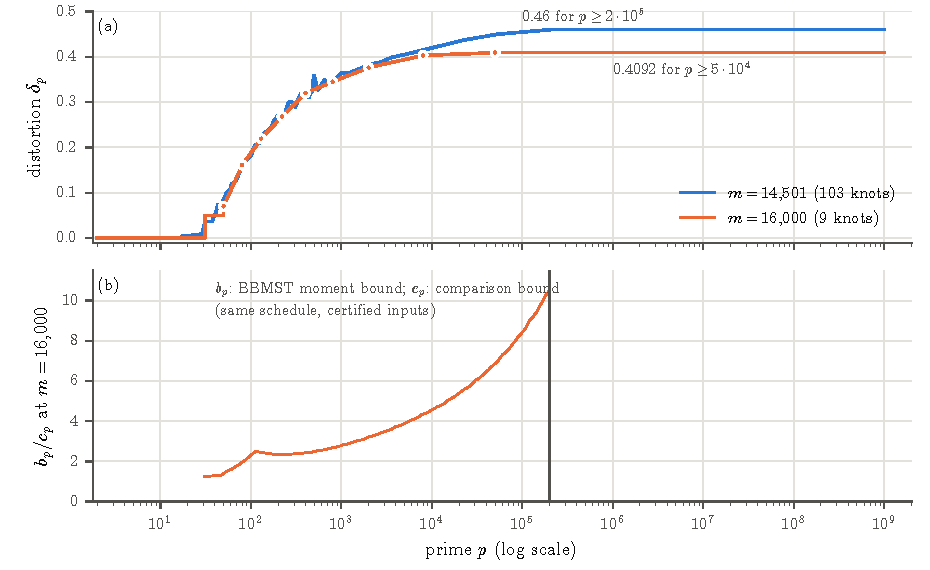
\includegraphics[width=\textwidth]{fig/schedule_gain.pdf}
  \caption{(a) The distortion schedules $\delta_p$ of the two certified runs; the dots are the knots of the schedule
  for $m=\MzeroLean$. (b) The ratio $b_p/c_p$ of the moment bound $b_p=\min\bigl(\E[U_p],\E[U_p^2]/(4\delta_p(1-\delta_p))\bigr)$
  of BBMST to the certified comparison bound $c_p$ at $m=\MzeroLean$, for $31\le p\le\PX$, with the same schedule;
  both are computed from certified quantities.}
  \label{fig:schedule}
\end{figure}

With the same schedule, the comparison bound is smaller than the moment bound of BBMST by a factor between
$\gainAmin$ and $\gainAmax$ for $31\le p<50$, between $\gainBmin$ and $\gainBmax$ for $50\le p<2{,}000$, and between
$\gainCmin$ and $\gainCmax$ for $2{,}000\le p\le\PX$ (\cref{fig:schedule}(b)).

%% =====================================================================================
\section{The certified computations}\label{sec:computation}
%% =====================================================================================

\subsection{Arithmetic with directed rounding}\label{sec:rounding}

The certified checkers \path{certificate-14501/src/rigx.c} (for \cref{thm:main}) and \path{src/rigcert.c} (for
\cref{thm:lean}) are single C files that implement \cref{sec:evaluation} in IEEE-754 double precision with directed
rounding. The first was derived from the second and keeps all of its conventions. (Separate implementations in
fixed-point integer arithmetic are part of the formalizations of \cref{thm:main,thm:lean}; see
\cref{sec:certified-formal,sec:lean}.) The conventions
are as follows; \cref{app:rounding} lists the rounding direction of the quantities.
\begin{itemize}
\item The processor is switched to round-upward mode once and stays there, so every $+,-,\times,/$ returns an
  upper bound for the exact result of its operands. Lower bounds are computed as
  $\mathrm{RD}(x\circ y)=-\mathrm{RU}(-(x\circ y))$. Square roots are corrected to the required direction by an
  exact fused-multiply-add sign test.
\item No library transcendental function enters any bound. Powers $q^{-a}$ are formed by repeated division,
  $(a+1)^\theta$ by repeated multiplication and a directed square root, and the logarithms in the test of
  \cref{prop:bbmst61} are replaced by rigorous lower bounds from a truncated $\operatorname{artanh}$ series with
  positive terms. Library functions such as \code{log}, \code{pow} and \code{sqrt} are called only to evaluate the
  schedule and to choose free parameters (enumeration cut-offs, the split point $y$ of \cref{sec:SBH}, table sizes).
\item Quantities that enter a total with a plus sign are rounded up; quantities that are subtracted, such as the
  partial Euler sums in \eqref{eq:EU}, the thresholds $\beta$ in \cref{sec:SBH} and the enumerated mass in
  \eqref{eq:AB-bound}, are rounded down. Differences that would cancel badly are replaced by algebraically identical
  sums of nonnegative terms, such as the lost-mass recursion \eqref{eq:lost} and the suffix sums \eqref{eq:suffix}.
\item The decimal output is formatted from integers, so the printed totals are themselves upper bounds.
\item A start-up self-test aborts if directed rounding or the negation idiom does not behave as expected, or if
  constant folding in round-to-nearest is detected. The sources forbid \code{-ffast-math} and turn off
  floating-point contraction.
\end{itemize}

\emph{The schedule and the tilts.} The value $d_p$ of the schedule is evaluated once per prime in round-to-nearest
(with \code{libm}'s logarithm) and stored. The tilt used everywhere afterwards, in the random numbers $s_{p'}$ for
$p'>p$ and in $T_X$, is the double $\hat\nu_p=\mathrm{RU}\bigl(1/\mathrm{RD}(1-d_p)\bigr)\ge1/(1-d_p)$. We therefore
apply \cref{thm:criterion} and \cref{prop:bbmst61} with the schedule $\delta_p:=1-1/\hat\nu_p\ge d_p$, for which
$\nu_p=\hat\nu_p$ exactly. The bounds at level $p$ use $t\le d_p\le\delta_p$ in (i) and $d=\min(d_p,\frac12)\le\delta_p$
in (ii) and (iii), so they are admissible. All $\delta_p$ are at most $0.46+10^{-15}<\frac12$. The programs assert
$\hat\nu_p\le p$ at every prime, and $t\le d_p$ holds by construction (\code{rigx.c} uses $t=d_p$) or is asserted
(\code{rigcert.c}).

\emph{A rounding gap and its repair.} An audit found one rounding-direction flaw in \code{rigcert.c}: $(p-1)^2$ was
formed by converting an exact integer to a double, which can round \emph{up} in round-upward mode for
$p\ge94{,}906{,}267$, where $(p-1)^2>2^{53}$, although it is used as a divisor of upper bounds (in the second moments
and in the factors of $T_X$). These bounds could therefore be low by one unit in the last place. The program now uses
$\mathrm{RD}((p-1)^2)$ and reproduces the certified output for \cref{thm:lean} bit for bit
(\code{src/CERT\_NOTES.md}); \code{rigx.c} had the repair from the start.

\subsection{The certificate for \cref{thm:main}}\label{sec:certified}

The certified run for $m=\Mzero$ (command in \cref{app:reproduce}) prints
\[
  \eta_{\mathrm{up}}=\etaMainTwelve\qquad(A=\blockAMain,\ B=\blockBMain,\ C=\blockCMain),
\]
where $A$, $B$ and $C$ are the contributions of the primes $p<50$, $50\le p\le\PX$ and $\PX<p\le\PmaxMain$. The total
is the double $\etaMainFull$ (\code{\etaMainHex}), rounded up in the twelfth decimal. The program also prints
$k=\pi(\PmaxMain)=\kPrimesMain$, the upper bound $T_{\mathrm{up}}=\TupMain$ for $T_{\PmaxMain}$, and the quantities of the
test of \cref{prop:bbmst61}. \Cref{tab:budget} shows the budget by prime ranges, next to that of the certificate for
\cref{thm:lean}, and \cref{app:budget} gives finer breakdowns. About $\shareBelowTwoK\%$ of the budget is spent at the
primes below $2{,}000$.

\begin{table}[ht]
\centering
\caption{Where the budget goes. Certified contributions of the prime ranges for $m=\Mzero$
($P_{\max}=\PmaxMain$) and $m=\MzeroLean$ ($P_{\max}=\Pmax$); the second column gives the number of primes (for the
last two rows, for $m=\Mzero$ and for $m=\MzeroLean$). Every entry is rounded up in the sixth decimal; the totals
are the certified values of $\eta_{\mathrm{up}}$, rounded up.}
\label{tab:budget}
\small
% generated by make_figures.py from certificate-14501/output and logs/ -- do not edit
\begin{tabular}{@{}lrrr@{}}
\toprule
primes & number & $m=14{,}501$ & $m=16{,}000$ \\
\midrule
$p<17$ & 6 & 0.037108 & 0.034611 \\
$17\le p<50$ & 9 & 0.197793 & 0.195961 \\
$50\le p<200$ & 31 & 0.364896 & 0.365330 \\
$200\le p<2{,}000$ & 257 & 0.314659 & 0.312354 \\
$2{,}000\le p<20{,}000$ & 1{,}959 & 0.072697 & 0.071735 \\
$20{,}000\le p\le 2\cdot 10^5$ & 15{,}722 & 0.011319 & 0.010886 \\
$2\cdot 10^5<p\le P_{\max}$ & 50{,}829{,}550 / 11{,}060{,}953 & 0.001458 & 0.006511 \\
\midrule
total, $p\le P_{\max}$ & 50{,}847{,}534 / 11{,}078{,}937 & 0.999927 & 0.997385 \\
\bottomrule
\end{tabular}

\end{table}

\begin{proof}[Proof of \cref{thm:main}]
Apply \cref{prop:bbmst61} with $m=\Mzero$, $X=\PmaxMain$, the schedule $\delta_p=1-1/\hat\nu_p$ of \cref{sec:rounding}
for $p\le X$ and $\delta_p=\frac12$ for $p>X$, and $c_p$ the per-prime costs computed by the certified program. Each
$c_p$ is an upper bound for one of the quantities (i)--(iii) of \cref{thm:criterion}: for $p<17$ the first moment,
which is (i) with $t=0=\delta_p$, and otherwise a comparison bound with $t=d_p\le\delta_p$, multiplied by a margin
factor larger than $1$. The program certifies $\eta=\sum_{p\le X}c_p\le\etaMainTwelve<1$, and with
$\mu_{\mathrm{lo}}=\mathrm{RD}(1-\eta_{\mathrm{up}})\ge\muLoMain$ it certifies
\[
  \frac{T_X}{1-\eta}\le f_{\mathrm{up}}=\mathrm{RU}\Bigl(\frac{T_{\mathrm{up}}}{\mu_{\mathrm{lo}}}\Bigr)\le\fUpMain,
  \qquad
  (\log k+\log\log k-3)^2k\ge\critLoMain,
\]
where $k=\kPrimesMain\ge10$ and the logarithms are bounded below as in \cref{app:rounding}. Since
$\fUpMain<\critLoMain$, \cref{prop:bbmst61} applies. Therefore no family of congruences with distinct moduli, all at
least $\Mzero$, covers $\Z$. \Cref{cor:main} follows, since a covering system with distinct moduli must then have a
modulus below $\Mzero$.
\end{proof}

The test of \cref{prop:bbmst61} passes with $f/(\log k+\log\log k-3)^2k\approx0.611$; it would hold for any
$\eta$ up to about $0.999955$ (\code{certificate-14501/xcheck/results/tail.out}), so the margin of the certificate is
about $2.8\cdot10^{-5}$ in $\eta$. The margin of \cref{thm:criterion} is not enough here, as noted in \cref{sec:tail}.

\subsection{The formal certificate for \cref{thm:main}}\label{sec:certified-formal}

The formal proof of \cref{thm:main} (\cref{sec:lean}) uses a second checker, written in Lean (\code{Checker2Impl}). It
evaluates the per-prime bounds as in \cref{sec:SBH,sec:tausplit}, for $m=\Mzero$, the primes $p\le X=\XFormal$ and
$t=\delta_p$, in fixed-point arithmetic with values $n/2^{62}$ and explicit directed rounding. The schedule is that of
the C certificate with the two knots at $p\ge5\cdot10^4$ set to $0.45$, rounded to multiples of $10^{-9}$, with
$\delta_p=0$ for $p<17$ and $\delta_p=\frac12$ for $p>X$.
\begin{itemize}
\item For $p<17$ it bounds $\E[U_p(s)]$, which is (i) with $t=\delta_p=0$.
\item For $17\le p<m/2$ it uses \cref{lem:SBH} in the lower-tail form
  $\E[(\tau_ST-\beta)^+]=\tau_S\E[T]-\E[\beta]+\E[(\beta-\tau_ST)^+]$. The last term involves the joint law of $(T,b)$
  only for $T\le\beta/\tau_S$, so this evaluation has neither lost mass nor exponent truncation. The enumeration of
  $s_S$ is pruned as in \cref{sec:SBH}, at the relative level $2^{-33}$, and the pruning bounds are added.
\item For $m/2\le p\le\PX$ it uses the $\tau$-split (\cref{lem:tausplit}) with the truncations of \cref{sec:lost},
  with the law of $\tau_S$ kept on $[0,2^{22}]$.
\item For $\PX<p\le X$ it takes the primes in blocks of relative width $2^{-13}$ and evaluates the $\tau$-split
  bound once per block, at the first element of the block, where it is largest.
\end{itemize}
The run certifies
\[
  \sum_{p\le X}c_p\le\etaFormal,\qquad T_X\le\TupFormal;
\]
the primes $p<17$, $17\le p\le\PX$ and $\PX<p\le X$ contribute $\etaFormalA$, $\etaFormalB$ and $\etaFormalC$.

\begin{proof}[Formal proof of \cref{thm:main}]
Apply \cref{thm:criterion} in the form of \cref{rem:criterion-sharp}, with $m=\Mzero$, $X=\XFormal$, the schedule above,
the per-prime costs $c_p$ of the Lean checker (each an upper bound for the quantity (i) with $t=\delta_p$), and the
constant $C_X=\frac{5941}{50000}$ of \cref{prop:tailtwo}. The left-hand side of the criterion is at most
\begin{multline*}
  \etaFormal+\frac{5941}{50000}\cdot\frac{\TupFormal}{\XFormal}\\
  \le\etaFormal+\tailFormal\le\totalFormal<1 .
\end{multline*}
Therefore no family of congruences with distinct moduli, all at least $\Mzero$, covers $\Z$.
\end{proof}

The whole argument, including the soundness of every step of the checker and the tail estimate, has been checked by
Lean's kernel. The only trusted step is the compiled evaluation of the checker (\cref{sec:lean}), which takes about ten
minutes and $2.6$ GB. The margin is $\slackFormal$. For $m=14{,}500$ a floating-point prototype of the same checker
gives $\sum_pc_p>1$ on its own, so $\Mzero$ is also the limit of the formal version of the method. On the way, the
same development certified $m=14{,}600$ with $X=\Pmax$ and the tail of \cref{prop:tail} (total $\totalLeanTwo$), and
$m=14{,}505$ with $X=10^9$ (total $\totalLeanThree$). The C program \path{certificate-14501/src/rigx.c}, run at
$m=14{,}600$ and $X=\Pmax$ with matching settings, agrees with the Lean checker's sum $\sum_{p\le X}c_p$ to within
$10^{-6}$.

\subsection{The certificate for \cref{thm:lean}}\label{sec:certified-lean}

The certified run for $m=\MzeroLean$ prints
\[
  \eta_{\mathrm{up}}=\etaCertTwelve\qquad(A=\blockA,\ B=\blockB,\ C=\blockC),
\]
for the primes $p<50$, $50\le p\le\PX$ and $\PX<p\le\Pmax$. The total is the double $\etaCertFull$
(\code{\etaCertHex}), rounded up in the twelfth decimal. The program also prints $k=\pi(\Pmax)=\kPrimes$ and the upper
bound $T_{\mathrm{up}}=\Tup$ for $T_{\Pmax}$.

\begin{proof}[Proof of \cref{thm:lean}]
Apply \cref{thm:criterion} with $m=\MzeroLean$, $X=\Pmax\ge2^{27}$, the schedule $\delta_p=1-1/\hat\nu_p$ of
\cref{sec:rounding} for $p\le X$ and $\delta_p=\frac12$ for $p>X$, and $c_p$ the per-prime costs computed by the
certified program, each of which is an upper bound for one of the quantities (i)--(iii). The program certifies
$\sum_{p\le X}c_p\le\etaCertTwelve$ and $T_X\le T_{\mathrm{up}}<\TupCeil$. Hence the left-hand side of
\eqref{eq:criterion} is at most
\[
  \etaCertTwelve+\frac{100}{189}\cdot\frac{\TupCeil}{\Pmax}
  \le\etaCertTwelve+\tailElem<\etaElem<1 .
\]
Therefore no family of congruences with distinct moduli, all at least $\MzeroLean$, covers $\Z$.
\end{proof}

The criterion of BBMST gives an independent confirmation of the tail. With
$\mu_{\mathrm{lo}}=\mathrm{RD}(1-\eta_{\mathrm{up}})\approx\muLo$, the program certifies
$T_X/(1-\eta)\le f_{\mathrm{up}}\le\fUp$ and $(\log k+\log\log k-3)^2k\ge\critLo$, so \cref{prop:bbmst61} applies as
well, with $f/(\log k+\log\log k-3)^2k\approx0.043$ (\code{logs/xcheck\_final.md}).

\subsection{Independent recomputation}\label{sec:xcheck}

\emph{The certificate for \cref{thm:main}.} Two independent checks were made.
\begin{enumerate}[label=(\arabic*)]
\item \emph{Cross-check by independently written code} (\code{certificate-14501/xcheck/}). The programs of the
  recomputation of the certificate for \cref{thm:lean} described below, which were written independently of both
  checkers, were rerun with the new schedule (only their schedule header was changed), together with a new program
  for the large primes that uses no code of \code{rigx.c}. For each prime they compute a rigorous interval
  $[\mathrm{lo},\mathrm{hi}]$ for the exact value of the level bound. \Cref{tab:xcheck-main} summarizes the results:
  the certified cost is at least $\mathrm{hi}$ at every prime compared, and the total of the upper ends for
  $\PX<p\le\PmaxMain$ is below the certified $C$.
\item \emph{Independent referee.} An AI agent acting as a referee checked the mathematics of
  \cref{sec:SBH,sec:tausplit,sec:lost} by hand; brute-forced the identity of \cref{lem:SBH} with exact rationals on
  $36{,}840$ random pairs $(p,s)$ at all $\nPrimesSBH$ primes where it is used, including cases with $y$ itself a
  prime of $B$ and with $v_q\ge2$ for $q\in B$ (no mismatch); audited the rounding directions and the lost-mass
  accounting; and recomputed every level bound for all primes up to $\PmaxMain$ with separately written programs (an
  exact complement identity with a pruned enumeration for $p<\firstTau$, and a logarithmic-grid law of $\tau(s)$ with
  its own sieve for the larger primes), with exact-rational and $60$-digit spot checks. It obtained the rigorous
  interval $[\refEtaLo,\refEtaHi]$ for the sum of the level bounds, found the certified cost at or above its upper
  bound at every prime (at every level up to $\PX$ and at every $500$-th prime beyond, where the per-prime costs are
  recorded), reproduced the run bit for bit on macOS with Apple clang and with GNU gcc, and found no errors. Its remaining
  remarks were that the trust base includes \cite[Theorem~6.1]{BBMST} and that the bound for the largest primes is
  conservative (\cref{sec:tausplit}).
\end{enumerate}

\begin{table}[ht]
\centering
\caption{The cross-check of the certificate for \cref{thm:main}. Here $\mathrm{hi}$ is the upper end of an
independent rigorous interval for the exact level bound, and ``cost'' is the certified cost, including the margins of
\cref{sec:eval-overview}.}
\label{tab:xcheck-main}
\small
\begin{tabular}{@{}>{\raggedright\arraybackslash}p{0.3\textwidth}>{\raggedright\arraybackslash}p{0.64\textwidth}@{}}
\toprule
check & result\\
\midrule
schedule, all $\nPrimesPX$ primes $p\le\PX$ & relative deviation from a $40$-digit evaluation at most $4.5\cdot10^{-16}$;
  $\hat\nu_p\ge1/(1-d_p)$ everywhere\\
first moments, $p<17$ & exact rational values; at most the certified cost at all $6$ primes\\
S/B/H levels, $17\le p\le\lastSBH$ & all $\nPrimesSBH$ primes, with two different splits whose intervals always overlap;
  $0$ violations; cost/hi $\in[1+9.2\cdot10^{-7},\,1+9.6\cdot10^{-7}]$\\
$\tau$-split levels, $\firstTau\le p\le\PX$ & all $\nPrimesTauPX$ primes, with a direct law of $\tau(s)$; $0$ violations;
  cost/hi $\in[1+4.5\cdot10^{-5},\,1+1.2\cdot10^{-4}]$\\
$\tau$-split levels, $\PX<p\le\PmaxMain$ & $118{,}717$ primes compared (all $p\le\PX$ and every $500$-th prime beyond),
  $0$ violations; the upper ends summed over all $\nPrimesCMain$ primes give $0.0014578122\le C$\\
tail & $k=\kPrimesMain$ confirmed by a segmented sieve; $T_k=705974.98819$, below $T_{\mathrm{up}}$ by $1.0\cdot10^{-8}$
  relative; $f/(\log k+\log\log k-3)^2k=0.611$\\
\bottomrule
\end{tabular}
\end{table}

\emph{The certificate for \cref{thm:lean}.} Separately written code (\path{tests/xcheck_final/}), with its own
decomposition and its own outward rounding, recomputed this certificate (\path{logs/xcheck_final.md}); it reuses none
of the checker's machinery. For each of the $\nPrimesPX$ primes $p\le\PX$ and each candidate bound of the checker, it
computed a rigorous interval $[\mathrm{lo},\mathrm{hi}]$ for the exact value and checked
$c_p\ge\min_{\text{candidates}}\mathrm{hi}$ in exact rational arithmetic: there were $0$ violations and $0$
inconclusive cases, and the smallest relative margin, $1.4\cdot10^{-7}$ at $p=8009$, is seven times the width of the
interval there. For $31\le p<8000$ it uses the identity of \cref{lem:SBH}, and for $8000<p\le\PX$ a divisor-count
dynamic program on $[1,2^{20}]$ and the exact identity $\E[(\tau-x)^+]=\E\tau-x+\sum_{T\le x}(x-T)\P(\tau=T)$, which
needs no truncation; both are run in both rounding directions and agree with brute force on small instances. It also
reproduced the schedule bit for bit, the first and second moments (against $60$-digit values and direct double sums),
the total $0.0065107856047$ of the fractional-moment bounds over $(\PX,\Pmax]$ (against the checker's $\blockC$), the
prime count, the product $T_k=321051.3638366$ (the checker's $T_{\mathrm{up}}$ is larger by $2.2\cdot10^{-9}$ relative)
and the tail criterion. It also measures the slack of the cruder evaluation. The sum over $p\le\PX$ of the exact values of the
best candidate bounds is $\xcheckExact$, against the checker's $\sumCostPX$; the difference, about $\xcheckSlack$, is
almost entirely at $p\ge50$. The recomputations check numbers, not mathematics: the comparison theorem and the
reduction of \cref{sec:loss} are outside their scope. Their interval code relies on the compiler honouring directed
rounding (it passes its own self-tests and was cross-validated against brute force and $60$-digit arithmetic).

\subsection{Tests}\label{sec:tests}

\emph{The checkers' formulas.} On small instances, independent Python programs compare every quantity that
\code{rigcert.c} computes with brute-force enumeration of $s$ (with a rigorous bracket for the pruned part), with exact
rational arithmetic (for $\E[U_p]$ and $\E[U_p^2]$, via a different decomposition) and with $50$-digit arithmetic (for
the products $\E[\tau(s)^\theta]$) (\code{tests/cert/run\_small.sh}). The instances use the knot schedule and the
constant band of the final run, values $\delta>\frac12$, and tiny truncation parameters that force every tail path.
There were no failures over $308$ comparison-bound candidates, $84$ moment-bound candidates and the first and second
moments at every prime; on two larger instances, $108$ primes of exact moments and $828$ pairs $(p,\theta)$ of
$50$-digit products agreed. Earlier validations on other configurations, including $431$ exact prime checks, are
described in \code{src/CERT\_NOTES.md}. For \code{rigx.c}, plain enumeration of $s$ was compared with $42$ cases at
$m=300$ and $m=1000$, including settings that force every truncation and lost-mass path
(\code{certificate-14501/validation/}); the certified values were always at least the lower end of the brute-force
bracket, and inside the bracket with the default settings. At $m=\MzeroLean$ with the schedule of \cref{thm:lean},
\code{rigx.c} agrees with the exact intervals of the recomputation above to within $10^{-9}$ relative at the S/B/H
levels and lies inside the intervals at the others.

\emph{The comparison theorem.} About $10^6$ randomized, exhaustive and adversarial tests (\code{tests/review/})
found no violation of \cref{lem:onecoord}, \cref{thm:comparison} and \cref{lem:pointwise}. They compare the
theorem with the exact worst case over all $\nu$-bounded product measures (computed by a backward bathtub recursion),
include an exhaustive search over all families of at most three cylinders on $\Z/4\times\Z/3$, and simulate the
measures of BBMST exactly on small moduli, checking \cref{lem:F1}, the kernel bounds of \cref{lem:kernel},
\cref{lem:F3} and each inequality in the proof of \cref{thm:perprime}.

\emph{Proof review.} Separate AI referee passes checked each step of the proof of the comparison theorem and of the
reduction, and the new steps of \cref{sec:SBH,sec:tausplit,sec:lost}; they found no gap, and their presentational
suggestions have been incorporated. No human has refereed the argument yet.

\subsection{Run times and reproducibility}\label{sec:runtimes}

The certified run for \cref{thm:main} takes $87$--$93$ seconds on one core of an Apple M3 Max and about $1.2$~GB of
memory (for the sieve up to $10^9$). Rebuilt from the published source, it reproduces the certified result lines and
the per-prime dump bit for bit; the referee reproduced them on macOS with Apple clang and with GNU gcc. On Linux
(x86-64, glibc, GNU gcc at \code{-O0} and at \code{-O2}, which agree) the run also certifies, with the same result
line; the last digits of the certified value and $503$ of the $119{,}644$ per-prime costs in the dump differ, by at
most about $2\cdot10^{-12}$ relative, because of the logarithm (see below). The cross-check of
\cref{tab:xcheck-main} takes about $29$ minutes on one core. The certified run for \cref{thm:lean} takes $156.6$
seconds of CPU time on one core (\code{logs/timing.txt}) and is also reproduced bit for bit
(\code{logs/repro16k.txt}). Bit-for-bit reproduction requires floating-point contraction to be off and the same
\code{libm} logarithm, which is used only to evaluate the schedule; another \code{libm} may move some $d_p$ by one
unit in the last place. The last digits of the output would then change, but the certificates would remain valid,
since any schedule is admissible and the checkers use their own values consistently.

\subsection{Formal verification}\label{sec:lean}
% Status (2026-09-28): complete for thm:main, thm:lean, thm:squarefree, thm:sf23, thm:sf7type, thm:odd, thm:odd2;
% source DELIV/lean/README.md (coordinator's axiom audits).

\Cref{thm:main,thm:lean} have been formally verified in Lean~4 (v4.34.1) with Mathlib, each modulo one
\code{native\_decide} evaluation. The development is in the folder \path{lean/} of the accompanying files, and
\path{lean/README.md} describes the build and the audit. The root theorems, in
\path{lean/MinModulus/Checker2Sound/Final14501.lean} and \path{lean/MinModulus/Main/Main.lean}, are
\begin{alltt}\small
theorem MinModulus.Checker2Sound.not_covers_14501 \{\(\iota\) : Type*\} [Fintype \(\iota\)]
    (d : \(\iota\) \(\to\) \(\mathbb{N}\)) (a : \(\iota\) \(\to\) \(\mathbb{Z}\)) (hd : Function.Injective d)
    (hm : \(\forall\) i, \MzeroNum \(\le\) d i) :
    \(\exists\) x : \(\mathbb{Z}\), \(\forall\) i, \(\neg\) ((d i : \(\mathbb{Z}\)) \(\mid\) x - a i)
theorem MinModulus.not_covers \{\(\iota\) : Type*\} [Fintype \(\iota\)]
    (d : \(\iota\) \(\to\) \(\mathbb{N}\)) (a : \(\iota\) \(\to\) \(\mathbb{Z}\)) (hd : Function.Injective d)
    (hm : \(\forall\) i, \MzeroLeanNum \(\le\) d i) :
    \(\exists\) x : \(\mathbb{Z}\), \(\forall\) i, \(\neg\) ((d i : \(\mathbb{Z}\)) \(\mid\) x - a i)
\end{alltt}
Neither contains \code{sorry}. For each, \code{\#print axioms} lists only \code{propext}, \code{Classical.choice},
\code{Quot.sound} and one auxiliary axiom introduced by \code{native\_decide}:
\begin{center}\small\code{MinModulus.Tail2.check2T14501\_eq\_true.\_native.native\_decide.ax\_1\_1}\\
\code{MinModulus.CheckerImpl.check\_eq\_true.\_native.native\_decide.ax\_1\_1}\end{center}
respectively. Each states that one closed Boolean (\code{check2T14501}, respectively \code{check}) evaluates to
\code{true}. The trust base is therefore Lean's kernel together with the compiled evaluation of this Boolean. That
takes about ten minutes and $2.6$ GB for \code{check2T14501}, and about $50$ seconds for \code{check}. It trusts
Lean's compiler and runtime, including the arbitrary-precision arithmetic on natural numbers. The code of both
checkers contains no \code{implemented\_by}, \code{extern}, \code{unsafe} or \code{partial} declarations; the only
compiler rewrites are two \code{@[csimp]} lemmas, which are proved equalities. The evaluation of \code{check} has been
re-run from a fresh file. The whole development, including every native evaluation, has also been rebuilt from a fresh
copy of the sources (with the Mathlib build shared), in about eleven minutes. Both gave the same results and the
same axioms.

\emph{The formalization of \cref{thm:main}.} It reuses the modules \code{Arith}, \code{Distortion},
\code{Comparison}, \code{Smooth}, \code{Tail} and \code{Main} of the first formalization unchanged, including the
certificate interface \code{Cert}. It also reuses the checker's arithmetic, sieve and first-moment code with their
soundness proofs. New are the following parts.
\begin{itemize}
\item The checker \code{Checker2Impl}, which implements \cref{sec:certified-formal}.
\item The mathematics of its quantities, in \code{Checker2Math}:
  \begin{itemize}
  \item \cref{lem:SBH,lem:tausplit} and the domination $\tau(s)\le2^{\sum v_q}$;
  \item the lower-tail identity;
  \item the joint law of $(T,b)$ and the law of the exponent sum;
  \item the depth-first enumeration and its pruning bound.
  \end{itemize}
\item A code-level soundness proof, \code{Checker2Sound}, covering:
  \begin{itemize}
  \item the dynamic programs, their states and the tables;
  \item the S/B/H and $\tau$-split costs;
  \item the loops and the blocks;
  \item the assembly of the certificate interface (\code{E.run2\_sound}).
  \end{itemize}
\item The sharpened tail estimate \cref{prop:tailtwo} and the corresponding form of \cref{thm:criterion}
  (\code{Tail2}), and the certificate \code{check2T14501\_eq\_true}.
\end{itemize}
The soundness theorem \code{E.run2\_sound} holds for all parameters of the checker that satisfy four decidable side
conditions. A certificate for another $m$, or another schedule, therefore needs only a new \code{native\_decide}
evaluation.

\emph{Structure of the first formalization.} The whole development has $255$ files and about $52{,}700$ lines,
counting the formalizations of \cref{thm:main,thm:lean,thm:squarefree,thm:sf23,thm:sf7type,thm:odd,thm:odd2} but not
the $194$ generated modules that embed and check the certificate data of \cref{thm:sf7type}. Of these, $64$ files and
about $18{,}400$ lines belong to the first formalization. \Cref{tab:lean} lists the modules and their correspondence with this paper. The first formalization
follows the paper, with two differences: it uses the
comparison theorem only for the hinge functions, since the other bounds are obtained from the hinge with
$t=\delta_p$ by pointwise inequalities on the aligned side, and it treats the primes above $X=\Pmax$ by
\cref{prop:tail}, so that it needs neither \cite[Theorem~6.1]{BBMST} nor Dusart's estimate.

\emph{The checker of the first formalization.} The numerical certificate for \cref{thm:lean} is produced by an
independent implementation of the checker in core Lean (\code{CheckerImpl}), not a transcription of
\code{src/rigcert.c}. It works in fixed point, with values $n/2^{62}$ and explicit directed rounding; it uses
$t=\delta_p$ only, with $\delta_p$ an exact rational (a multiple
of $10^{-9}$ obtained from the same knots) and exact rational tilts; and for $\PX<p\le\Pmax$ it processes the primes
in blocks, taking the factors of each block at its first prime, with $\theta\in\{2,\frac52,3\}$. It certifies
$\sum_{p\le\Pmax}c_p\le\etaLean$ and $T\le\TupLean$ (slightly larger than in the C program, because of the blocks),
so that the total with the tail term $\frac{100}{189}T/X=\tailLean$ is $\totalLean<1$. A code-level soundness proof
(\code{CheckerSound}) shows that the checker's loops and arrays bound the true per-prime losses (invariants of the
dynamic programs, semantics of the enumeration, the blocks) and assembles them into the certificate
\code{Cert \MzeroLeanNum{} (2*10\^{}8) \(\delta\) c T} consumed by \code{MinModulus.Main.not\_covers\_of\_cert}, whose
conditions correspond to those of \cref{thm:criterion} with $t=\delta_p$. The squarefree theorem of
\cref{sec:squarefree} is formalized in the same way, with its own checker. \Cref{thm:sf23} is formalized as
\code{MinModulus.SliceCert.not\_covers\_sf3\_23smooth}, an instance of a general theorem
\code{not\_covers\_of\_slices} for certificates of the kind described in \cref{sec:squarefree} (any start moduli and
residual primes), which uses only the three standard axioms; the certificate itself is checked by one
\code{native\_decide} evaluation (\code{check23\_eq\_true}, about $70$ seconds).

\emph{The formalization of \cref{thm:sf7type}.} It is the theorem
\code{MinModulus.SquarefreeM7.not\_covers} in the module \code{SquarefreeM7}; its hypotheses are those of
\code{MinModulus.not\_covers} above, together with \code{Squarefree (d i)} and $7\le{}$\code{d i}. It has four parts, which interact only through propositions fixed in advance.
\begin{itemize}
\item The reduction to the nine types, the symmetries and the classes modulo $30$ (\code{Reduction}), checked
  entirely by the kernel.
\item The per-level bound for families with repetitions at every level, with the tail of \cref{thm:sf7type}: the
  levels $7$, $11$ and $13$ with the Jensen splits and the exact terms (including the split by the class of the
  modulus $390$), the grouped bound with power-of-two thresholds for the other levels up to $2^{31}$, and
  \cref{prop:tail} beyond (\code{Bound}).
\item The tail coefficients: a sieve up to $2^{31}$ and the Poisson--binomial recursions with upward rounding, with a
  proof that they bound the true sums, run in $16$ chunks for each of the two schedules (\code{Coef}).
\item A checker in core Lean with exact integer arithmetic, about $1.6$ times slower than the C verifier, with its
  soundness proof, and the nine certificates, converted to an exact format and embedded as data ($446$~MB in $83$
  chunks; \code{Check}, \code{Data}, \code{Cert}).
\end{itemize}
\code{\#print axioms} lists \code{propext}, \code{Classical.choice}, \code{Quot.sound} and $124$ auxiliary axioms of
\code{native\_decide}: $83$ for the certificate chunks, $9$ for the level-$7$ covers of the nine types and $32$ for the
tail coefficients. The reduction and the analytic part use only the three standard axioms. A build of the whole
development from scratch takes about $80$ minutes on $24$ threads, almost all of it in the certificate chunks.

\emph{What is not formalized.} The C certificate of \cref{thm:main} (\cref{sec:certified}) and
\cite[Theorem~6.1]{BBMST}, which it uses, are not formalized; the formal proof does not need them. \Cref{thm:odd} is
formalized (\cref{sec:odd}), and so is \cref{thm:odd2}; \cref{thm:sf29,thm:sf6smooth} and the results of
\cref{sec:rings} are not.

\begin{table}[ht]
\centering
\caption{Modules of the Lean formalization (\code{lean/MinModulus/}) and the corresponding results of this paper.}
\label{tab:lean}
\small
\begin{tabular}{@{}lr>{\raggedright\arraybackslash}p{0.69\textwidth}@{}}
\toprule
module & lines & contents\\
\midrule
\code{Arith} & $679$ & setup of a family of congruences: $Q$, the primes and levels, the Chinese remainder
  theorem, the sets $B_\ell$, \cref{lem:unionbound,lem:pointwise,lem:enlargement}\\
\code{Distortion} & $646$ & the measures \eqref{eq:rule}, kernels and tilts, \cref{lem:F1,lem:F2,lem:F3},
  \cref{prop:F4,lem:kernel}\\
\code{Comparison} & $710$ & \cref{lem:greedy,lem:onecoord} (by duality), \cref{prop:rectangles,lem:vlaw}, and
  \cref{thm:comparison} for hinges\\
\code{Smooth} & $2142$ & the tilted law of $s$, $U_p(s)$, the moments $\E[\tau(s)^\theta]$, hinge bounds, monotone
  coupling in the exponent caps\\
\code{Tail} & $354$ & \cref{prop:tail}\\
\code{Main} & $613$ & the certificate interface \code{Cert}, \code{not\_covers\_of\_cert} (\cref{thm:perprime} with
  $t=\delta_p$, \cref{thm:criterion}), the final theorem\\
\code{CheckerImpl} & $1269$ & the executable checker and \code{check\_eq\_true} (by \code{native\_decide})\\
\code{CheckerMath} & $4094$ & the mathematics of the checker's quantities: laws of $\tau(s_A)$ and $\tau(s_B)$,
  the split of \cref{lem:AB}, the comparison bound, first and fractional moments\\
\code{CheckerSound} & $6201$ & code-level soundness: loop and array invariants, enumeration, dynamic programs,
  blocks, and the assembly of the certificate (\code{CheckerSound.D.cert\_16000})\\
\code{Squarefree} & $1649$ & \cref{thm:squarefree}, with its own checker and soundness proof\\
\midrule
\multicolumn{3}{@{}l}{\emph{formalization of \cref{thm:main}}}\\
\code{Checker2Impl} & $1139$ & the executable checker of \cref{sec:certified-formal}\\
\code{Checker2Math} & $2155$ & \cref{lem:SBH,lem:tausplit} in the form of the hinge loss, the lower-tail identity, the
  joint law of $(T,b)$, the law of the exponent sum, the enumeration and its pruning bound\\
\code{Checker2Sound} & $6604$ & code-level soundness: dynamic programs, tables, the S/B/H and $\tau$-split costs,
  loops and blocks, the generic soundness theorem \code{E.run2\_sound}, and the final theorem
  \code{not\_covers\_14501}\\
\code{Tail2} & $2022$ & \cref{prop:tailtwo}, the criterion with the sharpened tail, and the certificate
  \code{check2T14501\_eq\_true} (by \code{native\_decide})\\
\midrule
\code{Odd} & $4381$ & \cref{thm:odd,thm:odd2}: the chain for restricted moduli, the per-case weights, a checker for
  the $\tau$-split bounds with excluded and capped primes, its soundness, and nine \code{native\_decide}
  certificates\\
\code{SliceCert} & $3138$ & \cref{thm:sf23}: the class decomposition modulo $30$, the per-level bound for families
  with repetitions, certificate records and the branch-and-bound tree with symmetries, the start-case check, and
  \code{check23\_eq\_true} (by \code{native\_decide})\\
\code{SquarefreeM7} & $14950$ & \cref{thm:sf7type}: the reduction to the nine types, the per-level bound with the
  refinements at $7$, $11$ and $13$ and the tail, the tail coefficients up to $2^{31}$, the exact checker and its
  soundness (and $194$ generated modules: the certificate data and $124$ \code{native\_decide} checks)\\
\bottomrule
\end{tabular}
\end{table}
% CHECK: the Lean checker's totals are from DELIV/lean/README.md and SCRATCH/agents/checkerimpl/full_final.out
%        (0.997384786285, 321095.49941797, tail 0.000849458994, total 0.998234245279); they are not under DELIV/logs.

%% =====================================================================================
\section{Limits of the method}\label{sec:limits}
%% =====================================================================================

The proof bounds the true loss $P_i(B_i)$ by a chain of steps: the union bound $\alpha_i\le\min(1,U_i)$ in the fibre
(\cref{lem:unionbound}); the pointwise hinge step, which discards the cap $\alpha_i\le1$ (\cref{lem:pointwise});
the comparison theorem, which aligns the progressions and tilts the measure (\cref{thm:comparison}); the enlargement
to all admissible moduli (\cref{lem:enlargement}); and the union bound over the levels in \cref{prop:F4}. On top of
this comes the slack of the numerical evaluation. In this section we discuss how much each step loses. Statements
labelled Proposition are proved. Statements labelled Observation are numerical findings from floating-point
experiments (Monte Carlo sampling at $m=16{,}000$, and exact computations and adversarial searches on small
analogues, and computations of the exact level bounds near $m=14{,}500$); they are not proofs and are not used
anywhere in the proofs of \cref{thm:main,thm:lean}.

\subsection{Steps that are sharp}

\emph{Alignment and tilt.} By \cref{prop:sharp}, \cref{thm:comparison} is attained by aligned cylinders and a
suitable $\nu$-bounded measure, so no better inequality holds for the whole class of $\nu$-bounded product measures.

\emph{Enlargement.} \Cref{lem:enlargement} loses nothing for a family that contains all admissible moduli
$m'p^j\ge m$ with $m'\mid Q_{i-1}$, up to the truncation of the exponents, which disappears as the exponents
$\gamma_j$ grow. Such families can be used at all levels at once, since moduli with different largest prime factors
are automatically distinct.

\emph{The redistribution rule.} By \cref{rem:rule-optimal}, given $P_{i-1}$ the rule \eqref{eq:rule} minimizes the
loss at level $i$ among all rules that preserve the marginal and multiply masses by at most $\nu_i$.

\emph{The tilt in practice.} \Cref{prop:sharp} uses a measure that is chosen freely, whereas $P_{i-1}$ is produced
by the rule \eqref{eq:rule}. The following observation shows that the tilt is nevertheless essentially attained.

\begin{observation}[the tilt is realized by nested shells]\label{obs:tilt}
Consider configurations of \emph{nested shells}, in which the progressions of every level are aligned at a common
centre, so that points that are heavily covered at one level are heavily covered at every smaller level as well. In
such a configuration the fibres of rich points receive, at each earlier level, the tilt
$\min(\nu_q,1/(1-\alpha_q))$ of \eqref{eq:rule}. Monte Carlo sampling ($10^6$ importance-sampled paths) at
$m=16{,}000$ with the final schedule, for $p\le2\cdot10^4$, gives the following totals of the per-level bound
$\E[(U_p-\delta_p)^+]/(1-\delta_p)$: $0.970$ with the full tilt $\nu_q$ (the bound used in the proof, whose exact value
is $0.9703$), $0.767$ without tilt ($\nu_q=1$), and $0.953$ with the tilt that nested shells realize. So the tilt
accounts for about $0.20$ of the budget, most of it at $200\le p<8{,}000$, and all but about $0.017$ of it is realized
by an actual configuration.
\end{observation}
% Source of the Observations: SCRATCH/agents/r9-tightness/FINDINGS.txt (sections 2, 3, 6 and the summary; the
% per-range Monte Carlo table there gives full tilt / no tilt / capped totals 0.97012 / 0.76699 / 0.75264 for
% p <= 2e4), SCRATCH/agents/r8-global-accounting/results.txt.  All numerical, floating point.

\subsection{The cap cannot be used by convex functionals}

The pointwise step replaces $(\min(1,U)-\delta)^+$ by the hinge $(U-t)^+$, which grows beyond $U=1$. The next
proposition shows that no convex functional can do better, so that the comparison theorem cannot exploit the cap
$\alpha\le1$.

\begin{proposition}\label{prop:cap}
Let $0<\delta<1$ and $f_\delta(u)=(\min(1,u)-\delta)^+/(1-\delta)$ for $u\ge0$. Let $\varphi\colon[0,\infty)\to\R$ be
convex with $\varphi\ge f_\delta$. Then for every random variable $W\ge0$ with $\E W<\infty$,
\[
  \E\varphi(W)\ge\min\Bigl(1,\ \min_{0\le t\le\delta}\frac{\E(W-t)^+}{1-t}\Bigr).
\]
\end{proposition}

\begin{proof}
Replacing $\varphi$ by its lower semicontinuous regularization, which is still convex, still majorizes the
continuous function $f_\delta$ and is not larger than $\varphi$, we may assume that $\varphi$ is continuous. Let
$\sigma^*=1/(1-\delta)$, the slope of $f_\delta$ on $[\delta,1]$, and let $\varphi'_-(1)$ be the left derivative at $1$.

\emph{Case $\varphi'_-(1)\le\sigma^*$.} Put $\sigma=\varphi'_-(1)$; it is a subgradient at the interior point $1$, so
$\varphi(u)\ge\varphi(1)+\sigma(u-1)\ge1+\sigma(u-1)$ for all $u\ge0$, because $\varphi(1)\ge f_\delta(1)=1$. Also
$\varphi\ge0$. If $\sigma\le0$, then $\varphi\ge1$ on $[0,1]$, and $\varphi\ge f_\delta=1$ on $[1,\infty)$, so
$\E\varphi(W)\ge1$. If $0<\sigma\le\sigma^*$, put $t=1-1/\sigma\le\delta$; then
$\varphi(u)\ge\max(0,\sigma(u-t))=\max(0,(u-t)/(1-t))$. For $t\ge0$ this gives $\E\varphi(W)\ge\E(W-t)^+/(1-t)$.
For $t<0$ it gives $\E\varphi(W)\ge(\E W-t)/(1-t)$, a convex combination of $\E W$ and $1$, which is at least
$\min(1,\E W)$, the bound for $t=0$.

\emph{Case $\varphi'_-(1)>\sigma^*$.} The continuous convex function $\psi(u)=\varphi(u)-\sigma^*u$ attains its
minimum over $[0,1]$ at some $u^*<1$, because $\psi'_-(1)>0$. It is then a global minimum on $[0,\infty)$: if
$\psi(v)<\psi(u^*)$ for some $v>1$, convexity would give $\psi(w)<\psi(u^*)$ for $w\in(u^*,1]$. Hence
$\varphi(u)\ge\varphi(u^*)+\sigma^*(u-u^*)$ for all $u\ge0$. Since
$\varphi(u^*)\ge f_\delta(u^*)\ge(u^*-\delta)/(1-\delta)$, this gives $\varphi(u)\ge(u-\delta)/(1-\delta)$, and together
with $\varphi\ge0$, $\varphi(u)\ge(u-\delta)^+/(1-\delta)$. So $\E\varphi(W)\ge\E(W-\delta)^+/(1-\delta)$.
\end{proof}

Applied to $W=U^{\mathrm{al}}$, \cref{prop:cap} says that the bound of \cref{thm:perprime}, minimized over $t$ and
capped at $1$, is the best that \cref{thm:comparison} can give for the loss. The cap does matter at the aligned
configuration: there the excess $\E[(U-1)^+]/(1-\delta)$ charged beyond the cap amounts to $0.217$ (numerical),
about $22\%$ of the budget for $p\le2\cdot10^4$, and between $20\%$ and $26\%$ of the budget of each range of primes.
An adversary, however, can spread the progressions apart.

\begin{observation}[spreading]\label{obs:spread}
In exact computations on small analogues (moduli built from the primes up to $7$ or up to $13$, with the worst
$\nu$-bounded measure and adversarial residues found by simulated annealing), spreading the progressions recovers
most of the gap between the capped aligned value and the per-level bound: between $59\%$ and $100\%$, depending on
the instance. At $m=16{,}000$, the explicit spreadings we tried recover at most about $15\%$ of the cap excess at the
prime $101$. Whether the true per-level worst case at this scale is much below the bound of \cref{thm:perprime} is
open.
\end{observation}

\subsection{Cross-level accounting}

The union bound over the levels in \cref{prop:F4} is not an identity, and its slack has a simple exact description.

\begin{proposition}\label{prop:live}
Call $x\in\Z_{Q_{i-1}}$ \emph{alive} if $x\notin\bigcup_{j<i}B_j$. Then
\[
  P_n\Bigl(\bigcup_{i=1}^nB_i\Bigr)=\sum_{i=1}^n\frac{\E_{P_{i-1}}\bigl[(\alpha_i-\delta_i)^+\,\one\{x\text{ alive}\}\bigr]}{1-\delta_i}.
\]
\end{proposition}

\begin{proof}
The union is the disjoint union of the sets $B_i\setminus\bigcup_{j<i}B_j$, which are $Q_i$-measurable, so by
\cref{lem:F1} its $P_n$-measure is $\sum_iP_i(B_i\setminus\bigcup_{j<i}B_j)$. The set $\bigcup_{j<i}B_j$ is
$Q_{i-1}$-measurable, so each fibre $F(x)$ either lies inside it or is disjoint from it. Hence
$P_i(B_i\setminus\bigcup_{j<i}B_j)=\sum_{x\text{ alive}}P_i(F(x)\cap B_i)$, and the computation in the proof of
\cref{lem:F3} finishes the proof.
\end{proof}

Thus $\sum_iP_i(B_i)$ also charges the losses on fibres that are already covered at an earlier level. In the nested
shells of \cref{obs:tilt} this happens systematically: the same rich points are charged at every level.

\begin{observation}[double counting]\label{obs:double}
On two small exact analogues (moduli dividing $2^43^25\cdot7$ and $2^53^35\cdot7$, with schedules optimized for the
bound of \cref{thm:perprime}), the per-level bounds sum to $1.0241$ and $0.9938$; simulated annealing finds systems
with $\sum_iP_i(B_i)=0.9934$ and $0.9511$, so the per-level chain loses only $0.031$ and $0.043$. Simulated annealing aimed
directly at $P_n(\bigcup_iB_i)$ finds at most $0.907$ and $0.886$: the double counting, about $0.07$ to $0.09$ of the budget, exceeds the
whole per-level slack. At $m=16{,}000$, in a Monte Carlo model of nested shells, the configuration that attains the
per-level bounds simultaneously (sum of capped losses about $0.74$ for $p\le2\cdot10^4$) newly covers only
$0.10$--$0.16$ of the mass. We did not obtain a rigorous improvement of the certified total from this observation.
\end{observation}

\subsection{The slack of the evaluation and the reach of the method}\label{sec:reach}

For the certificate of \cref{thm:lean} the evaluation itself is lossy. At $m=\MzeroLean$, with the schedule of that
certificate, the exact values of the level bounds (computed with \code{rigx.c}, without margins) total $0.982431$ over
the primes up to $\Pmax$, against the certified $\etaCertTwelve$. About $0.0097$ of the difference comes from
$50\le p<200$, where the decomposition of \cref{lem:AB} is inexact once $N_1>53$, and about $0.0053$ from $p>\PX$,
where the fractional-moment bounds are about six times the exact values. The exact evaluation of
\cref{sec:SBH,sec:tausplit,sec:lost} removes this slack. The following observation, from computations of the exact
level bounds without the safety margins and with heuristically optimized schedules, describes the reach of the
per-level method.

\begin{observation}[the frontier]\label{obs:frontier}
With the exact evaluation and the schedule of \cref{thm:lean}, the total crosses $1$ near $m=14{,}780$. With the
$\nKnotsMain$-knot schedule of \cref{thm:main} and $P_{\max}=10^9$, the total is $0.9999918$ at $m=14{,}500$ and
$1.0000041$ at $m=14{,}499$. One damped per-prime Newton step on the schedule (a schedule with $3{,}241$ knots)
gives $0.99996996$ at $m=14{,}498$ and $1.00002227$ at $m=14{,}495$. A total below $1$ is not
yet a proof: at $P_{\max}=10^9$ the test of \cref{prop:bbmst61} needs
$1-\eta\ge T_X/(\log k+\log\log k-3)^2k\approx4.5\cdot10^{-5}$, which is why $m=14{,}498$ to $14{,}500$ are not
certified. We estimate the frontier of the per-level method at $m^*\approx14{,}496\pm3$. Near $m=14{,}500$ the total is
a step function of $m$ that increases on average by about $0.015$ for each decrease of $1{,}000$ in $m$, and about
$\shareBelowTwoK\%$ of the budget is spent at the primes below $2{,}000$, where the level bound is now evaluated
exactly.
\end{observation}

A sharper evaluation of the same level bounds can therefore gain only a few units in $m$. Going substantially
further requires changing the method itself: a different rule for redistributing the removed mass, an accounting
across levels that exploits \cref{prop:live} (for instance a comparison theorem for the sub-stochastic kernels
$K_j\one\{\text{alive}\}$), or a non-convex treatment of the cap.
% Sources: the final report of SCRATCH/agents/r7-method-limit (frontier, 0.982431, 0.0097, 0.0053, 14,780, slope)
%          and certificate-14501/README.md (frontier data); share of p < 2000 from certificate-14501/output/dump.
% CHECK: sources disagree on the sensitivity of eta to m.  SCRATCH/agents/CONTEXT.md and r9-tightness/FINDINGS.txt
%        give "about 0.0085 per 1000" near m = 16,000; the r7 report measures about 0.015 per 1000 near m = 14,500
%        and says that 0.0085 does not hold there (r8-global-accounting/results.txt also gave about 0.015).
%        The text follows the r7 report.  (DELIV/README.md, "Limits of the approach", now also gives the limit
%        m ~ 14,500 and the frontier m* ~ 14,496, as here.)


\subsection*{Acknowledgements}
This work was carried out with substantial assistance from AI systems (Anthropic's Claude), including the design
of the computation, the proofs, independent re-verification and the Lean formalization; all computations are
reproducible from the accompanying code. The results have been checked by independent recomputation, by randomized,
exhaustive and brute-force tests and by separate AI referee passes over the proofs and the computations.
\Cref{thm:main,thm:lean} have been formally verified in Lean~4 modulo one \texttt{native\_decide} evaluation each.
None of the results has yet been refereed by human experts. We thank the
authors of \cite{BBMST}, whose distortion method and careful exposition this work builds on.
% TODO(acknowledgements): add funding and personal acknowledgements.

%% References.  Bibliographic data from SCRATCH/agents/r10-literature/refs.bib unless noted.
\begin{thebibliography}{99}

\bibitem{BBMST}
P.~Balister, B.~Bollob\'as, R.~Morris, J.~Sahasrabudhe and M.~Tiba,
\emph{On the {E}rd\H{o}s covering problem: the density of the uncovered set},
Invent. Math. \textbf{228} (2022), no.~1, 377--414. arXiv:1811.03547.

\bibitem{BBMST2021ES}
P.~Balister, B.~Bollob\'as, R.~Morris, J.~Sahasrabudhe and M.~Tiba,
\emph{The {E}rd\H{o}s--{S}elfridge problem with square-free moduli},
Algebra Number Theory \textbf{15} (2021), no.~3, 609--626. arXiv:1901.11465.

\bibitem{BurchardHajaiej2006}
A.~Burchard and H.~Hajaiej,
\emph{Rearrangement inequalities for functionals with monotone integrands},
J. Funct. Anal. \textbf{233} (2006), no.~2, 561--582.

\bibitem{CFT2025}
M.~Cummings, M.~Filaseta and O.~Trifonov,
\emph{An upper bound for the minimum modulus in a covering system with squarefree moduli},
Acta Math. Hungar. \textbf{175} (2025), no.~1, 1--25. arXiv:2211.08548.

\bibitem{Dusart1999}
P.~Dusart,
\emph{The $k$th prime is greater than $k(\ln k+\ln\ln k-1)$ for $k\ge2$},
Math. Comp. \textbf{68} (1999), 411--415.

\bibitem{Erdos1950}
P.~Erd\H{o}s,
\emph{On integers of the form $2^k+p$ and some related problems},
Summa Brasil. Math. \textbf{2} (1950), 113--123.

\bibitem{FFKPY2007}
M.~Filaseta, K.~Ford, S.~Konyagin, C.~Pomerance and G.~Yu,
\emph{Sieving by large integers and covering systems of congruences},
J. Amer. Math. Soc. \textbf{20} (2007), no.~2, 495--517.

\bibitem{FilasetaKalogirou2026}
% RESOLVED 2026-09-27 (source files corrected): DELIV/README.md writes "T. Kalogirou"; the arXiv text (SCRATCH/lit/2407.15280.txt) and refs.bib give
%        Alexandros Kalogirou, as here.
M.~Filaseta and A.~Kalogirou,
\emph{Covering systems with the sum of the reciprocals of the moduli close to $1$},
Trans. Amer. Math. Soc. \textbf{379} (2026), 4945--4972. arXiv:2407.15280.

\bibitem{Gibson2009}
D.~J.~Gibson,
\emph{A covering system with least modulus $25$},
Math. Comp. \textbf{78} (2009), 1127--1146.

\bibitem{HalberstamRoth1966}
H.~Halberstam and K.~F.~Roth,
\emph{Sequences}, Oxford University Press, 1966; reprinted by Springer, 1983. Rogers' theorem: pp.~242--244.

\bibitem{Hough2015}
R.~Hough,
\emph{Solution of the minimum modulus problem for covering systems},
Ann. of Math. (2) \textbf{181} (2015), no.~1, 361--382. arXiv:1307.0874.

\bibitem{KKL2024}
J.~Klein, D.~Koukoulopoulos and S.~Lemieux,
\emph{On the $j$th smallest modulus of a covering system with distinct moduli},
Int. J. Number Theory \textbf{20} (2024), no.~2, 471--479. arXiv:2212.01299.

\bibitem{Kucheriaviy2026}
P.~Kucheriaviy,
\emph{An analogue of {R}ogers' theorem on sieving in commutative rings}, preprint (2026), arXiv:2603.14080.

\bibitem{Lewis1996}
E.~Lewis,
\emph{Infinite covering systems of congruences which don't exist},
Proc. Amer. Math. Soc. \textbf{124} (1996), 355--360.

\bibitem{LWWY2024}
H.~Li, B.~Wang, C.~Wang and S.~Yi,
\emph{On covering systems of polynomial rings over finite fields},
Proc. Amer. Math. Soc. \textbf{152} (2024), no.~9, 3731--3742. arXiv:2308.05378.

\bibitem{LWWY2025}
H.~Li, B.~Wang, C.~Wang and S.~Yi,
\emph{On {E}rd\H{o}s covering systems in global function fields},
J. Number Theory \textbf{266} (2025), 269--280. arXiv:2402.03810.

\bibitem{LiWangYi2026}
H.~Li, B.~Wang and S.~Yi,
\emph{On the minimum modulus problem in number fields}, preprint (v2, 2026), arXiv:2302.05946.

\bibitem{Nielsen2009}
P.~P.~Nielsen,
\emph{A covering system whose smallest modulus is $40$},
J. Number Theory \textbf{129} (2009), no.~3, 640--666.

\bibitem{Owens2014}
T.~Owens,
\emph{A covering system with minimum modulus $42$}, Master's thesis, Brigham Young University, 2014.

\bibitem{Simpson1986}
R.~J.~Simpson,
\emph{Exact coverings of the integers by arithmetic progressions},
Discrete Math. \textbf{59} (1986), 181--190.
% Lemma 2.3 is Rogers' theorem (credited by T. Tao, blog comment of 5 March 2026, linking this article).

\bibitem{Sun2006}
Z.-W.~Sun,
\emph{Finite covers of groups by cosets or subgroups},
Internat. J. Math. \textbf{17} (2006), no.~9, 1047--1064. arXiv:math/0501451.

\bibitem{TaoRogers2026}
T.~Tao,
\emph{Rogers' theorem on sieving}, blog post, What's new, 19 January 2026,
\url{https://terrytao.wordpress.com/2026/01/19/rogers-theorem-on-sieving/}.

\bibitem{BWang2026}
B.~Wang,
\emph{Bounds for {E}rd\H{o}s covering systems in global function fields},
Int. J. Number Theory \textbf{22} (2026), no.~6, 1327--1336. arXiv:2408.10460.

\end{thebibliography}


\appendix
%% =====================================================================================
\section{The distortion schedules}\label{app:schedule}
%% =====================================================================================

Both certified programs evaluate the schedule in the same way, in double precision with round-to-nearest. Given
knots $(q_0,\delta_0),\dots,(q_n,\delta_n)$ and a threshold $P_D$, the value at a prime $p\ge P_D$ is $d_p=\delta_0$
if $\log p\le\log q_0$, $d_p=\delta_n$ if $\log p\ge\log q_n$, and otherwise
\[
  d_p=(1-u)\,\delta_l+u\,\delta_{l+1},\qquad u=\frac{\log p-\log q_l}{\log q_{l+1}-\log q_l},
\]
where $l$ is the first index with $\log p\le\log q_{l+1}$. For $m=\Mzero$, $P_D=17$ and $d_p=0$ for $p<17$; the
$\nKnotsMain$ knots are listed in \cref{tab:knots-main} (and in \path{certificate-14501/schedule/sched_14501.json}). For $m=\MzeroLean$, $P_D=50$, $d_p=0.05$ for $31\le p<50$ and
$d_p=0$ for $p<31$; the knots are listed in \cref{tab:knots}. The tilt is $\hat\nu_p=\mathrm{RU}(1/\mathrm{RD}(1-d_p))$,
and the distortion parameter of the proofs is $\delta_p=1-1/\hat\nu_p$ (\cref{sec:rounding}). In the programs' command
lines the schedules are given by the environment variables \code{KNOTS}, \code{PD}, \code{PSB} and \code{DSB}
(\cref{app:reproduce}).

\begin{table}[ht]
\centering
\caption{The $\nKnotsMain$ knots $(q,\delta)$ of the schedule for $m=\Mzero$.}
\label{tab:knots-main}
\footnotesize
% generated by make_figures.py from certificate-14501/schedule/sched_14501.json -- do not edit
\begin{tabular}{@{}rlrlrlrlrl@{}}
\toprule
$q$ & $\delta$ & $q$ & $\delta$ & $q$ & $\delta$ & $q$ & $\delta$ & $q$ & $\delta$ \\
\midrule
17 & 0.003750 & 19 & 0.005000 & 23 & 0.006250 & 29 & 0.008750 & 31 & 0.036250 \\
37 & 0.036250 & 41 & 0.055000 & 43 & 0.073750 & 47 & 0.072500 & 53 & 0.098150 \\
59 & 0.106800 & 61 & 0.119050 & 67 & 0.123650 & 71 & 0.131380 & 73 & 0.141290 \\
79 & 0.155230 & 83 & 0.160970 & 89 & 0.172510 & 97 & 0.178660 & 101 & 0.182540 \\
103 & 0.188650 & 107 & 0.198220 & 109 & 0.204200 & 113 & 0.206020 & 127 & 0.209837 \\
131 & 0.217630 & 137 & 0.223648 & 139 & 0.230595 & 149 & 0.234931 & 151 & 0.236266 \\
157 & 0.238825 & 163 & 0.241289 & 167 & 0.242881 & 173 & 0.249996 & 179 & 0.259213 \\
181 & 0.261402 & 191 & 0.264497 & 193 & 0.266549 & 197 & 0.269965 & 199 & 0.271361 \\
211 & 0.267464 & 223 & 0.264006 & 227 & 0.266240 & 229 & 0.268576 & 233 & 0.270686 \\
239 & 0.274956 & 241 & 0.279675 & 251 & 0.288000 & 257 & 0.296790 & 263 & 0.298855 \\
269 & 0.299341 & 271 & 0.301179 & 277 & 0.299224 & 281 & 0.300443 & 283 & 0.299810 \\
293 & 0.294209 & 307 & 0.288986 & 311 & 0.288947 & 313 & 0.290166 & 317 & 0.292580 \\
331 & 0.305797 & 337 & 0.309213 & 347 & 0.314773 & 349 & 0.315866 & 353 & 0.318408 \\
359 & 0.319916 & 367 & 0.318618 & 373 & 0.317664 & 379 & 0.316724 & 383 & 0.316106 \\
389 & 0.315191 & 397 & 0.313993 & 401 & 0.313793 & 409 & 0.315719 & 419 & 0.313074 \\
421 & 0.313538 & 431 & 0.310826 & 433 & 0.311277 & 439 & 0.310119 & 443 & 0.311003 \\
449 & 0.317314 & 457 & 0.319036 & 461 & 0.319885 & 463 & 0.322807 & 467 & 0.323646 \\
479 & 0.322280 & 487 & 0.337726 & 491 & 0.352946 & 499 & 0.358381 & 550 & 0.326000 \\
650 & 0.348360 & 800 & 0.342500 & 1{,}000 & 0.365220 & 1{,}200 & 0.363800 & 1{,}600 & 0.373440 \\
2{,}000 & 0.382450 & 2{,}700 & 0.387760 & 3{,}500 & 0.398100 & 5{,}000 & 0.404570 & 8{,}000 & 0.414350 \\
20{,}000 & 0.434850 & 50{,}000 & 0.449200 & 200{,}000 & 0.460000 & & & & \\
\bottomrule
\end{tabular}

\end{table}

\begin{table}[ht]
\centering
\caption{The knots of the schedule for $m=\MzeroLean$ and the corresponding tilts $\nu=1/(1-\delta)$.}
\label{tab:knots}
\small
\begin{tabular}{@{}lrrrrrrrrr@{}}
\toprule
$q$ & $50$ & $80$ & $130$ & $220$ & $400$ & $800$ & $2{,}000$ & $8{,}000$ & $50{,}000$\\
$\delta$ & $0.07$ & $0.1612$ & $0.2191$ & $0.2679$ & $0.3198$ & $0.345$ & $0.3762$ & $0.4031$ & $0.4092$\\
$\nu$ & $1.0753$ & $1.1922$ & $1.2806$ & $1.3659$ & $1.4702$ & $1.5267$ & $1.6031$ & $1.6753$ & $1.6926$\\
\bottomrule
\end{tabular}
\end{table}

%% =====================================================================================
\section{The budgets by prime ranges}\label{app:budget}
%% =====================================================================================

\Cref{tab:budget-main} refines \cref{tab:budget} for the certificate of \cref{thm:main}. For each range it gives the
number of primes, the range of $\delta_p$, the evaluation used (\cref{sec:eval-overview}), the certified total
$\sum c_p$ and the total of the certified first moments $\sum\E[U_p]$; the latter, $\sumMonePXMain$ over $p\le\PX$,
shows how much the distortion gains. For $p>\PX$ the program records the individual costs only at every $500$-th prime;
the row gives the certified total $C$.

\begin{table}[ht]
\centering
\caption{The certified budget for $m=\Mzero$ by prime ranges (from
\code{certificate-14501/output/dump\_14501.txt.gz}). All sums are rounded up in the sixth decimal.}
\label{tab:budget-main}
\small
% generated by make_figures.py from certificate-14501/output -- do not edit
\begin{tabular}{@{}lrllrr@{}}
\toprule
primes & number & $\delta_p$ & evaluation & $\sum c_p$ & $\sum\mathbb{E}[U_p]$ \\
\midrule
$2\le p<17$ & 6 & 0.0000 & first moment & 0.037108 & 0.037108 \\
$17\le p<31$ & 4 & 0.0038--0.0088 & S/B/H & 0.084588 & 0.090176 \\
$31\le p<50$ & 5 & 0.0363--0.0738 & S/B/H & 0.113205 & 0.147744 \\
$50\le p<100$ & 10 & 0.0982--0.1787 & S/B/H & 0.170212 & 0.318257 \\
$100\le p<200$ & 21 & 0.1825--0.2714 & S/B/H & 0.194684 & 0.613946 \\
$200\le p<500$ & 49 & 0.2640--0.3584 & S/B/H & 0.170063 & 1.053353 \\
$500\le p<1{,}000$ & 73 & 0.3277--0.3649 & S/B/H & 0.086675 & 1.038927 \\
$1{,}000\le p<2{,}000$ & 135 & 0.3638--0.3824 & S/B/H & 0.057922 & 1.246231 \\
$2{,}000\le p<7{,}253$ & 624 & 0.3825--0.4123 & S/B/H & 0.055035 & 2.771613 \\
$7{,}253\le p<20{,}000$ & 1{,}335 & 0.4123--0.4348 & $\tau$-split & 0.017663 & 2.570146 \\
$20{,}000\le p<50{,}000$ & 2{,}871 & 0.4349--0.4492 & $\tau$-split & 0.007209 & 2.588585 \\
$50{,}000\le p\le2\cdot 10^5$ & 12{,}851 & 0.4492--0.4600 & $\tau$-split & 0.004111 & 4.267893 \\
\midrule
$p\le 2\cdot 10^5$ & 17{,}984 & & & 0.998469 & 16.743973 \\
$2\cdot 10^5<p\le 10^9$ & 50{,}829{,}550 & 0.4600 & $\tau$-split & 0.001458 & \\
\bottomrule
\end{tabular}

\end{table}

\Cref{tab:budget-fine} does the same for the certificate of \cref{thm:lean}, with ranges between consecutive knots
of its schedule. It also gives the total $\sum b_p$ of the moment bounds of BBMST with the same schedule, and the ratio
$\sum b_p/\sum c_p$. Over $p\le\PX$ the first moments total $\sumMonePX$ and the moment bounds of BBMST $\sumBBPX$.

\begin{table}[ht]
\centering
\caption{The certified budget for $m=\MzeroLean$ between consecutive knots of the schedule (from
\code{logs/dump16k.txt}). All sums are rounded up in the sixth decimal.}
\label{tab:budget-fine}
\small
% generated by make_figures.py from logs/dump16k.txt and logs/cert16k.txt -- do not edit
\begin{tabular}{@{}lrlrrrr@{}}
\toprule
primes & number & $\delta_p$ & $\sum c_p$ & $\sum\mathbb{E}[U_p]$ & $\sum b_p$ & ratio \\
\midrule
$2\le p<31$ & 10 & 0.0000 & 0.120331 & 0.120331 & 0.120331 & 1.00 \\
$31\le p<50$ & 5 & 0.0500 & 0.110242 & 0.141679 & 0.141679 & 1.29 \\
$50\le p<80$ & 7 & 0.0813--0.1588 & 0.126588 & 0.214777 & 0.214777 & 1.70 \\
$80\le p<130$ & 9 & 0.1656--0.2163 & 0.117619 & 0.274202 & 0.270831 & 2.30 \\
$130\le p<220$ & 16 & 0.2198--0.2640 & 0.127195 & 0.441578 & 0.302992 & 2.38 \\
$220\le p<400$ & 31 & 0.2691--0.3191 & 0.123609 & 0.694849 & 0.291946 & 2.36 \\
$400\le p<800$ & 61 & 0.3199--0.3449 & 0.100274 & 0.978090 & 0.253437 & 2.53 \\
$800\le p<2{,}000$ & 164 & 0.3454--0.3762 & 0.082401 & 1.587360 & 0.238184 & 2.89 \\
$2{,}000\le p<8{,}000$ & 704 & 0.3762--0.4031 & 0.056629 & 2.956076 & 0.205359 & 3.63 \\
$8{,}000\le p<50{,}000$ & 4{,}126 & 0.4031--0.4092 & 0.022132 & 4.839575 & 0.113938 & 5.15 \\
$50{,}000\le p\le2\cdot 10^5$ & 12{,}851 & 0.4092 & 0.003860 & 4.128765 & 0.031409 & 8.14 \\
\midrule
$p\le 2\cdot 10^5$ & 17{,}984 & & 0.990874 & 16.377278 & 2.184877 & 2.21 \\
$2\cdot 10^5<p\le 2\cdot 10^8$ & 11{,}060{,}953 & 0.4092 & 0.006511 & & & \\
\bottomrule
\end{tabular}

\end{table}

%% =====================================================================================
\section{Rounding conventions of the checkers}\label{app:rounding}
%% =====================================================================================

This appendix summarizes \path{src/CERT_NOTES.md} and the header of \path{certificate-14501/src/rigx.c}.
Throughout, ``up'' means that the computed double is an upper bound for the exact value of the formula applied to the
computed inputs, and ``down'' a lower bound; the programs are in round-upward mode, and lower bounds use the negation
idiom of \cref{sec:rounding}.

\emph{Build and self-test.} The sources contain \code{\#pragma STDC FENV\_ACCESS ON} and \code{FP\_CONTRACT OFF}
and refuse to compile with \code{-ffast-math}. With GNU \code{gcc}, \code{-frounding-math} is required and the
programs must be built with \code{-O0}: \code{gcc} ignores the \code{FENV\_ACCESS} pragma and at \code{-O1} and above
may reuse a result across \code{fesetround}; Apple clang~21 honours the pragma at \code{-O2}. At start-up
the programs check that directed rounding and the negation idiom work and that no constant was folded in
round-to-nearest.

\emph{First moment.} By \eqref{eq:EU} and \eqref{eq:U-tau}, $\E[U_p(s)]=T_1/(p-1)-U_1$ with
$T_1=\prod_{q<p}(1+\hat\nu_q/(q-1))$ and $U_1=(p-1)^{-1}\sum_{d<N_1}\nu(d)c(d)/d$, the sum running over
$(p-1)$-smooth $d$. The product $T_1$ is rounded up and the subtracted partial sum $U_1$ down.

\emph{Second moment.} $\E[U_p(s)^2]$ is computed by a finite inclusion--exclusion formula of the form
$T/(p-1)^2-2T_1V/(p-1)+S$, where $T=\prod_{q<p}(1+\hat\nu_q(3q-1)/(q-1)^2)$ and $S$, a sum of nonnegative terms
(the programs assert $\hat\nu_q\le q$, which makes them nonnegative), are rounded up, and the subtracted quantities
$T_1$ and $V$ are rounded down (see \code{src/CERT\_NOTES.md} for the formula). The divisor $(p-1)^2$ is rounded down
(\cref{sec:rounding}), and the bound $\E[U_p^2]/(4d(1-d))$ has its denominator rounded down.

\emph{The exact evaluation} (\code{rigx.c}). All dynamic programs (for $T_H$, for $(T,b)$ given a profile, for
$\tau_s$ and for $(e_2,e_3)$) are positive linear maps, evaluated in round-upward mode with upper bounds for the
coefficients $\P(v_q=a)$, so every stored probability is an upper bound; in-place updates process the cells in an
order in which no updated cell is read again. The numbers $c(d)=1-p^{1-j_0(d)}$, $1-\frac1p$ and $t(p-1)$ are rounded
down, so the thresholds $\beta$ of \cref{sec:SBH} and $X$ of \cref{sec:tausplit} are lower bounds, and the hinges
are evaluated at these lower thresholds, which is valid since they are nonincreasing in the threshold. The suffix
sums \eqref{eq:suffix}, the bounds for the pruned subtrees, the lost masses \eqref{eq:lost} and the margin factors are
rounded up.

\emph{The simpler evaluation} (\code{rigcert.c}). The probabilities $\P(s_A)$ are carried as intervals through the
enumeration, and $U_A(s_A)$ is rounded up. The dynamic programs for the laws of $\tau(s_A)$ and $\tau(s_B)$ produce
upper bounds. In $G(k,u)$, the inputs $u$ and $k/(p-1)$ are rounded up and $c=1+(t-u)/a$ is rounded down, which is
safe because $G$ is monotone in each. The suffix sums for $\E[(\tau(s_B)-c)^+]$ are rounded up. The weights
$R_k=\P_{\mathrm{up}}(\tau(s_A)=k)-\P_{\mathrm{lo}}(\text{enumerated},\tau(s_A)=k)$ use the enumerated mass rounded
down. Finally $1-t$ is rounded down. The program enforces $t\le d_p$ exactly.

\emph{Fractional moments.} $q^{-a}$ is formed by repeated division in the required direction, $(a+1)^\theta$ by
repeated multiplication and a directed square root, and the series \eqref{eq:Etheta} is summed with the geometric
bound for its remainder given in \cref{sec:theta}. The constant $c_\theta$ is rounded up: the program uses the
unconstrained maximum $\frac{d}{\theta-1}(u^*)^{-\theta}$ with $u^*$ rounded down, or $1-d$ if the lower bound for $u^*$
exceeds $1$. The products $\E[\tau(s)^\theta]$ are rounded up, and $(p-1)^\theta$ and $1-d$ down.

\emph{Totals and the tail tests.} The total $\eta$ is the sum of the costs, rounded up. For
\cref{prop:bbmst61}, $\mu_{\mathrm{lo}}=\mathrm{RD}(1-\eta_{\mathrm{up}})$ and
$f_{\mathrm{up}}=\mathrm{RU}(T_{\mathrm{up}}/\mu_{\mathrm{lo}})$; the lower bound for $(\log k+\log\log k-3)^2k$ uses lower
bounds for the logarithms from the truncated series $\log y=2\sum_{i\ge0}z^{2i+1}/(2i+1)$, $z=(y-1)/(y+1)$, whose
terms are positive (with $\log2$ from the same series); the programs check $k\ge10$ and that the base is positive.
The logarithm lower bounds were compared with $50$-digit values.

\emph{Audits.} \code{rigcert.c} was derived from a floating-point prototype, which computed in round-to-nearest,
allowed $t$ slightly above $\delta_p$, could round the tilt below $1/(1-\delta_p)$, computed two truncation tails with
cancellation and truncated a series without bounding its remainder; all of this is corrected in the certified program,
which also refuses a debugging option that disables the tilt. A later audit found the rounding gap described in
\cref{sec:rounding}, which has been repaired.

%% =====================================================================================
\section{Reproducing the computations}\label{app:reproduce}
%% =====================================================================================

All paths are relative to the accompanying folder.

\emph{The certificate for \cref{thm:main}.} In \code{certificate-14501/}:
\begin{alltt}\footnotesize
./run_certificate.sh
\end{alltt}
builds \code{src/rigx.c} with \code{cc -O2 -frounding-math -ffp-contract=off} (\code{-O0} under GNU \code{gcc}),
runs \code{rigx \MzeroNum{} 1e9} with
the environment of the certified run (the $\nKnotsMain$ knots in \code{KNOTS}, \code{PD=17 PSB=0 DSB=0}; the accuracy
settings \code{EPS=1e-14 TINY=1e-30 HEFF=1e-16 TS=4194304 THM=1048576 TBUD=4194304}; the margins \code{MARGIN}$=2^{-20}$
and \code{MARGINL}$=$\code{MARGINL2}$=2^{-13}$), and compares the result lines with \code{output/cert\_14501.txt}
(line breaks added):
\begin{alltt}\footnotesize
m=14501 eta_up=0.999926855181 (A=0.234899856304 B=0.763569005991 C=0.001457990070)
  f_up=9.65174e+09 crit_lo=1.57871e+10 SUCCESS(certified)
CERT eta_up=0.99992685518076208 (0x1.fff669aac979p-1) T_up=705974.99523353134
  mu_lo=7.3144819237924708e-05 f_up=9651742974.9486885 crit_lo=15787081835.245779
  k=50847534 log_k_lo=17.744342183707648 loglog_k_lo=2.8760667148961203
\end{alltt}
It takes about $90$ seconds and $1.2$~GB. The cross-check of \cref{tab:xcheck-main} is run by
\path{xcheck/tools/run_xcheck.sh} with the same environment (about $29$ minutes), and \path{validation/run_bf.py} runs
the brute-force comparisons of \cref{sec:tests}.

\emph{The certificate for \cref{thm:lean}.} In \code{src/}:
\begin{alltt}\footnotesize
cc -O2 -frounding-math -ffp-contract=off -o rigcert rigcert.c -lm   # GNU gcc: -O0
K=50:0.07,80:0.1612,130:0.2191,220:0.2679,400:0.3198,800:0.345
K=$K,2000:0.3762,8000:0.4031,50000:0.4092
KNOTS=$K PSB=31 DSB=0.05 NOSTOP=1 \textbackslash
  ./rigcert 16000 50 200000 2e8 47 16 4.5 1000000 20000 0 -1 0.1 0.44 0.5
\end{alltt}
The arguments are, in order: $m$; the prime $50$ from which the knot schedule applies; the largest prime $\PX$
treated by the comparison bound; the largest prime $\Pmax$ treated explicitly; the largest prime $47$ allowed in
$s_A$; the constants $16$ and $4.5$ of the enumeration cut-off $X_p$; the caps $10^6$ and $2\cdot10^4$ of the
divisor-count tables; a verbosity flag; and an unused smooth schedule (ignored when \code{KNOTS} is set).
\code{PSB} and \code{DSB} give $\delta_p=0.05$ for $31\le p<50$; \code{NOSTOP} only disables an early exit. The
expected output (\code{logs/cert16k.txt}; line breaks added) is
\begin{alltt}\footnotesize
m=16000 eta_up=0.997384393974 (A=0.230571210247 B=0.760302397508 C=0.006510785610)
  f_up=1.22745e+08 crit_lo=2.83863e+09 SUCCESS(certified)
CERT eta_up=0.9973843939732947 (0x1.fea92ad34fe9cp-1) T_up=321051.36453405279
  mu_lo=0.0026156060267052972 f_up=122744542.28049764 crit_lo=2838631802.0518227
  k=11078937 log_k_lo=16.220556296052827 loglog_k_lo=2.7862793450197798
CERT stats: max_enumerated=12114518 t_clamped_to_delta=0
\end{alltt}
With \code{DUMP=file} the program writes the certified per-prime costs for $p\le\PX$ (\path{logs/dump16k.txt}).
The run takes about $2.5$ minutes on one core. The commands of the independent recomputation are listed at the end
of \code{logs/xcheck\_final.md} (code in \code{tests/xcheck\_final/}); \code{tests/cert/run\_small.sh} runs the
small-instance checks of \cref{sec:tests}, and the tests of the comparison theorem are the Python scripts in
\code{tests/review/}.

\emph{The results of \cref{sec:further}.} The scripts \path{squarefree/src/reproduce.sh} (about $30$ seconds) and
\path{odd-moduli/reproduce_all.sh} (about $10$ minutes), and the drivers listed in \path{applications/PACKAGE.md},
rerun the certificates of \cref{sec:squarefree,sec:odd,sec:rings}.

\emph{This paper.} In \code{paper/}, \code{make\_figures.py} regenerates \code{fig/} and \code{gen/} from the
certified outputs, and \code{tectonic main.tex} builds the paper.

\needspace{11\baselineskip}
\emph{Lean.} In \code{lean/}:
\begin{alltt}\footnotesize
lake exe cache get                                 # prebuilt Mathlib
lake build MinModulus.Checker2Sound.Final14501     # Theorem \ref{thm:main} (native check: about 10 min)
lake env lean MinModulus/Checker2Sound/Final14501Audit.lean   # axioms of the final theorems
lake build                                         # Theorem \ref{thm:lean} (native check: about 50 s)
lake build MinModulus.Squarefree.Main              # squarefree theorem
lake build MinModulus.Odd.Final                    # Theorem \ref{thm:odd} (native checks: 80 s each)
lake env lean MinModulus/CheckerSound/Audit.lean   # axioms of MinModulus.not_covers
lake env lean MinModulus/Squarefree/Axioms.lean    # axioms of the squarefree theorem
lake env lean MinModulus/Odd/FinalAudit.lean       # axioms of Theorem \ref{thm:odd}
\end{alltt}


\end{document}
